% Options for packages loaded elsewhere
\PassOptionsToPackage{unicode}{hyperref}
\PassOptionsToPackage{hyphens}{url}
\PassOptionsToPackage{dvipsnames,svgnames,x11names}{xcolor}
%
\documentclass[
  letterpaper,
  DIV=11,
  numbers=noendperiod]{scrartcl}

\usepackage{amsmath,amssymb}
\usepackage{iftex}
\ifPDFTeX
  \usepackage[T1]{fontenc}
  \usepackage[utf8]{inputenc}
  \usepackage{textcomp} % provide euro and other symbols
\else % if luatex or xetex
  \usepackage{unicode-math}
  \defaultfontfeatures{Scale=MatchLowercase}
  \defaultfontfeatures[\rmfamily]{Ligatures=TeX,Scale=1}
\fi
\usepackage{lmodern}
\ifPDFTeX\else  
    % xetex/luatex font selection
\fi
% Use upquote if available, for straight quotes in verbatim environments
\IfFileExists{upquote.sty}{\usepackage{upquote}}{}
\IfFileExists{microtype.sty}{% use microtype if available
  \usepackage[]{microtype}
  \UseMicrotypeSet[protrusion]{basicmath} % disable protrusion for tt fonts
}{}
\makeatletter
\@ifundefined{KOMAClassName}{% if non-KOMA class
  \IfFileExists{parskip.sty}{%
    \usepackage{parskip}
  }{% else
    \setlength{\parindent}{0pt}
    \setlength{\parskip}{6pt plus 2pt minus 1pt}}
}{% if KOMA class
  \KOMAoptions{parskip=half}}
\makeatother
\usepackage{xcolor}
\setlength{\emergencystretch}{3em} % prevent overfull lines
\setcounter{secnumdepth}{-\maxdimen} % remove section numbering
% Make \paragraph and \subparagraph free-standing
\makeatletter
\ifx\paragraph\undefined\else
  \let\oldparagraph\paragraph
  \renewcommand{\paragraph}{
    \@ifstar
      \xxxParagraphStar
      \xxxParagraphNoStar
  }
  \newcommand{\xxxParagraphStar}[1]{\oldparagraph*{#1}\mbox{}}
  \newcommand{\xxxParagraphNoStar}[1]{\oldparagraph{#1}\mbox{}}
\fi
\ifx\subparagraph\undefined\else
  \let\oldsubparagraph\subparagraph
  \renewcommand{\subparagraph}{
    \@ifstar
      \xxxSubParagraphStar
      \xxxSubParagraphNoStar
  }
  \newcommand{\xxxSubParagraphStar}[1]{\oldsubparagraph*{#1}\mbox{}}
  \newcommand{\xxxSubParagraphNoStar}[1]{\oldsubparagraph{#1}\mbox{}}
\fi
\makeatother


\providecommand{\tightlist}{%
  \setlength{\itemsep}{0pt}\setlength{\parskip}{0pt}}\usepackage{longtable,booktabs,array}
\usepackage{calc} % for calculating minipage widths
% Correct order of tables after \paragraph or \subparagraph
\usepackage{etoolbox}
\makeatletter
\patchcmd\longtable{\par}{\if@noskipsec\mbox{}\fi\par}{}{}
\makeatother
% Allow footnotes in longtable head/foot
\IfFileExists{footnotehyper.sty}{\usepackage{footnotehyper}}{\usepackage{footnote}}
\makesavenoteenv{longtable}
\usepackage{graphicx}
\makeatletter
\def\maxwidth{\ifdim\Gin@nat@width>\linewidth\linewidth\else\Gin@nat@width\fi}
\def\maxheight{\ifdim\Gin@nat@height>\textheight\textheight\else\Gin@nat@height\fi}
\makeatother
% Scale images if necessary, so that they will not overflow the page
% margins by default, and it is still possible to overwrite the defaults
% using explicit options in \includegraphics[width, height, ...]{}
\setkeys{Gin}{width=\maxwidth,height=\maxheight,keepaspectratio}
% Set default figure placement to htbp
\makeatletter
\def\fps@figure{htbp}
\makeatother
% definitions for citeproc citations
\NewDocumentCommand\citeproctext{}{}
\NewDocumentCommand\citeproc{mm}{%
  \begingroup\def\citeproctext{#2}\cite{#1}\endgroup}
\makeatletter
 % allow citations to break across lines
 \let\@cite@ofmt\@firstofone
 % avoid brackets around text for \cite:
 \def\@biblabel#1{}
 \def\@cite#1#2{{#1\if@tempswa , #2\fi}}
\makeatother
\newlength{\cslhangindent}
\setlength{\cslhangindent}{1.5em}
\newlength{\csllabelwidth}
\setlength{\csllabelwidth}{3em}
\newenvironment{CSLReferences}[2] % #1 hanging-indent, #2 entry-spacing
 {\begin{list}{}{%
  \setlength{\itemindent}{0pt}
  \setlength{\leftmargin}{0pt}
  \setlength{\parsep}{0pt}
  % turn on hanging indent if param 1 is 1
  \ifodd #1
   \setlength{\leftmargin}{\cslhangindent}
   \setlength{\itemindent}{-1\cslhangindent}
  \fi
  % set entry spacing
  \setlength{\itemsep}{#2\baselineskip}}}
 {\end{list}}
\usepackage{calc}
\newcommand{\CSLBlock}[1]{\hfill\break\parbox[t]{\linewidth}{\strut\ignorespaces#1\strut}}
\newcommand{\CSLLeftMargin}[1]{\parbox[t]{\csllabelwidth}{\strut#1\strut}}
\newcommand{\CSLRightInline}[1]{\parbox[t]{\linewidth - \csllabelwidth}{\strut#1\strut}}
\newcommand{\CSLIndent}[1]{\hspace{\cslhangindent}#1}

\KOMAoption{captions}{tablesignature}
\makeatletter
\@ifpackageloaded{caption}{}{\usepackage{caption}}
\AtBeginDocument{%
\ifdefined\contentsname
  \renewcommand*\contentsname{Table of contents}
\else
  \newcommand\contentsname{Table of contents}
\fi
\ifdefined\listfigurename
  \renewcommand*\listfigurename{List of Figures}
\else
  \newcommand\listfigurename{List of Figures}
\fi
\ifdefined\listtablename
  \renewcommand*\listtablename{List of Tables}
\else
  \newcommand\listtablename{List of Tables}
\fi
\ifdefined\figurename
  \renewcommand*\figurename{Figure}
\else
  \newcommand\figurename{Figure}
\fi
\ifdefined\tablename
  \renewcommand*\tablename{Table}
\else
  \newcommand\tablename{Table}
\fi
}
\@ifpackageloaded{float}{}{\usepackage{float}}
\floatstyle{ruled}
\@ifundefined{c@chapter}{\newfloat{codelisting}{h}{lop}}{\newfloat{codelisting}{h}{lop}[chapter]}
\floatname{codelisting}{Listing}
\newcommand*\listoflistings{\listof{codelisting}{List of Listings}}
\makeatother
\makeatletter
\makeatother
\makeatletter
\@ifpackageloaded{caption}{}{\usepackage{caption}}
\@ifpackageloaded{subcaption}{}{\usepackage{subcaption}}
\makeatother

\ifLuaTeX
  \usepackage{selnolig}  % disable illegal ligatures
\fi
\usepackage{bookmark}

\IfFileExists{xurl.sty}{\usepackage{xurl}}{} % add URL line breaks if available
\urlstyle{same} % disable monospaced font for URLs
\hypersetup{
  pdftitle={Leveraging SMS Messages to Predict Near Real-Time Alcohol Lapse in AUD Patients},
  pdfauthor={Coco Yu; John J. Curtin},
  pdfkeywords={Substance use disorders, Text sensing, Machine learning},
  colorlinks=true,
  linkcolor={blue},
  filecolor={Maroon},
  citecolor={Blue},
  urlcolor={Blue},
  pdfcreator={LaTeX via pandoc}}


\title{Leveraging SMS Messages to Predict Near Real-Time Alcohol Lapse
in AUD Patients}
\author{Coco Yu \and John J. Curtin}
\date{2024-12-09}

\begin{document}
\maketitle
\begin{abstract}
AUD remains a prevalent, lasting and costly problem in the United
States, yet few receive treatment due to barriers. Smart Digital
Therapeutics (DTx) are emerging as a promising tool to address these
barriers. They can potentially provide continuous risk monitoring and
individualized support through personal sensing and algorithms. This
study leverages SMS messages both three days and one week preceding a
lapse episode to predict next-day alcohol lapse. We recruited 138
participants (65 males; 121 Whites non-Hispanic) in early recovery with
a goal of abstinence. Self-reported alcohol use and text messages were
obtained during a 3-month period. We enginnered features from LIWC and
trained models with XGBoost. We used grouped, nested cross-validation to
select the best model configuration. The median auROC was .53 (95\% CI
{[}.52, .54{]}) for the best model across the 300 folds in the inner
loop. Our model performed consistently worse for people from different
underprivileged groups. We further calculated SHAP values and discovered
that social processes, social behaviors and second person pronoun emerge
as the most important features. Our study suggests that the LIWC model
fails to capture sufficient signal from SMS messages to be clinically
useful. Our next step is to use other natural language processing
methods to do feature engineering and compare the results with this
baseline LIWC model. Future studies should also consider other data
sources to improve model performance.
\end{abstract}


\section{Introduction}\label{introduction}

AUD remains a prevalent, lasting and costly problem in the United
States. According to 2022 NSDUH (National Institute on Alcohol Abuse and
Alcoholism, 2023a, 2023b), an estimate of 29.5 million (10.5\% of the
population) individuals aged 12 or older had AUD in 2022, which is
consistent with the estimates for 2021. AUD problems have also brought
huge economic burdens to the U.S., where excessive alcohol use has cost
\$223.5 billion in 2006 and \$249 billion in 2010 (Sacks et al., 2015).

Despite the high prevalence of AUD, limited number of individuals
receive alcohol treatments. Only a small portion (7.6\%) of individuals
aged 12 or older with AUD acquired alcohol use treatment in the past
year (National Institute on Alcohol Abuse and Alcoholism, 2023a, 2023b).
This low treatment acquisition rate is even more pronounced for
individuals from disadvantaged groups. Disparities in treatment-seeking
behavior based on race, gender, and age are evident (Abraham et al.,
2020; DiBartolo \& Jarosinski, 2017; Kaufmann et al., 2014; Schuler et
al., 2015; Verissimo \& Grella, 2017; Young et al., 2018). Only 6.6\% of
Black or African-American people, 3.8\% of people of two or more races,
and 4.8\% of Hispanic or Latino people with past-year AUD received
treatments (National Institute on Alcohol Abuse and Alcoholism, 2023a,
2023b). Women are less likely to obtain treatments compared to men, even
if they have equivalent level of perceived need for help (Gilbert et
al., 2019).

Several obstacles hinder people's utilization of treatment options.
Previous studies have identified that AUD patients face financial
barriers (Kaufmann et al., 2014; Schuler et al., 2015), lack of
knowledge or awareness (May et al., 2019; Probst et al., 2015; Williams
et al., 2018), social stigma (Finn et al., 2023; May et al., 2019;
Sedarous \& Flemming, 2023; Wallhed Finn et al., 2014), and geographical
barriers (Gregory et al., 2022) for accessing care. Individuals with
disadvantaged demographic background suffer from even heightened
barriers to treatment resources. Women with high severity of alcohol use
face larger fear of stigma compared to their male counterparts (Finn et
al., 2023). Provider availability in rural areas, fear of stigma, and
economic hardship all contribute to racial, gender and age disparities
in treatment seeking (Abraham et al., 2020; DiBartolo \& Jarosinski,
2017; Kaufmann et al., 2014; Schuler et al., 2015; Verissimo \& Grella,
2017; Young et al., 2018).

\subsection{DTx and smart DTx}\label{dtx-and-smart-dtx}

DTx is an effective and accessible supplemental tool that may partially
address extant challenges AUD patients face. DTx are evidence-based
health software that deliver assessments, interventions, and other
supports to patients to prevent, or manage a disease or disorder. They
can be utilized to provide continuing care for AUD patients after
treatment. Available evidence suggests they are generally effective for
mental health conditions including AUD and demonstrate clear clinical
advantages (Gustafson et al., 2014; Lecomte et al., 2020; Philippe et
al., 2022). Further, DTx may provide better access for hard-to-reach
populations, including those from socially marginalized group who
encounter increased barriers to access continuing support. They can
benefit patients from rural areas with low provider availability as they
are accessible remotely via mobile phones (Bucci et al., 2019; N.
Jacobson et al., 2023). DTx also have potentials to relieve barriers to
seek professional help resulting from stigma concerns as they can
facilitate anonymity and shorten the need for in-person interactions.
They are of lower costs compared to in person care and have the capacity
to be scalable.

The concept of ``smart'' DTx is emerging in recent years allowing us to
expand the benefits of DTx. Smart DTx comprises two key components.
First, they rely on personal sensing methods to collect data. Exemplary
measures include EMA, which actively prompts users to complete surveys
and can encompass desired questions on moods, social relationships,
stressful events, etc. Other relatively lower-burden sensing approaches
include the measurement of geolocation, phone call logs and text
messages collection. Those measures continuously and passively gather
information. They can thus provide longitudinal data that can be
temporally precise. Combined with self-reports that acquire contextual
information (e.g., levels of support users can obtain from their
frequently contacted people), they constitute rich data source for smart
DTx.

Second, smart DTx incorporates the rich dataset extracted from personal
sensing to build machine learning algorithms. The goal of such models is
to identify \emph{who} are at heightened risk for alcohol lapses,
\emph{when} they will lapse, and \emph{why} they are at increased risk.
Through the embedded algorithms, smart DTx can achieve two tasks: 1)
continuous AUD relapse risk-monitoring; and 2) individualized clinical
support when needed.

To enhance the effectiveness of smart DTx, those predictive modeling
should be accurate and temporally precise. In other words, they should
be capable of detecting increased lapse risks in a timely manner. These
predictions allow windows for subsequent support to prevent lapses
targeting a specific person. Notably, these functions are very important
given the dynamic nature of alcohol relapse. Some relapse factors (e.g.,
drinking partner, drinking behavior) are situated and can be fluctuating
over time. They usually occurs before an episode of alcohol use (Chih et
al., 2014). They can be elusive to therapists' attention due to
infrequent visits, highlighting importance of sustained monitoring to
prevent lapses. AUD is a chronic, dynamic and temporally varying disease
where patients face constant challenges of relapsing after abstinence
(Andersson et al., 2019; Scott et al., 2005; Witkiewitz \& Marlatt,
2007). This requires constant monitoring over time and timely
intervention when necessary.

Importantly, the machine learning models should also predict well among
individuals from disadvantaged groups. One of the key benefits of DTx is
that they partially address barriers utilizing professional help by
providing 24/7/365, affordable, personalized support. They are
particularly beneficial to marginalized groups who have low rates of
utilizing treatment options due to these treatment barriers. However,
they might exacerbate health inequity if embedded algorithms perform
relatively worse for less privileged groups. To improve algorithm
fairness among different demographic subgroups, the models can
incorporate a diverse representation of sample to complete model
training. On the other hand, the models should derive more ``fair''
features. For example, models might be biased if they leverage
theory-driven features only. These features might be biased against
disadvantaged groups because they depend on decades of research on White
males.

To develop such algorithms, we must first identify a clinically relevant
outcome to predict. This outcome should be clearly and precisely defined
across individuals, easy to measure, and with high temporal precision.
Relapse, which usually refers to the return of a symptomatic behavior,
is hard to quantify due to its multidimensional nature and temporal
coarseness (Miller, 1996). One potential conceptualization of alcohol
relapse is linked to problems of use. Nonetheless, negative consequences
are multifaceted and can therefore be burdensome to collect. It is also
unclear what the onset of problems are. Another possible outcome is
quantity of alcohol use. However, this measure is not temporally precise
because there will be a time lag between onset of drinking and the last
drink completed. Levels of drinking might also mean differently for
individuals with different AUD severity, which makes it hardly
generalizable across individuals. Alternatively, in this study, we
utilize lapse (i.e., a single episode of alcohol use) as our primary
outcome variable. Lapses are easy to define, have a clear onset, and are
also clinically meaningful. They can serve as an early warning sign of
failure to sustain a desired behavioral change (Chung \& Maisto, 2006;
Marlatt \& Donovan, 2005). Research has also shown that initial lapse
and frequent lapses are the associated with enhanced risk of relapse
(Högström Brandt et al., 1999; Witkiewitz \& Marlatt, 2004).

Next, we need to determine what inputs to use for our prediction model.
The features should be easy to measure and feasible. The widespread
availability of smartphones has rendered constant data collection with
DTx attainable. Data collection procedure should not be unduly
burdensome to users to ensure that sensing is sustainable. Previous
research has established satisfying acceptability of active self-report
measures such as EMA and even more willingness to use passive sensing
measures (Wyant et al., 2024). The features should also be
well-validated. For example, GPS tracking has high accuracy in locating
individuals and is temporally precise. Text sensing captures precisely
the interactions between users and other individuals via SMS.

Smart DTx algorithms should also incorporate features that are
interpretable and can map on to current interventions. Exemplary
features that are highly interpretable include those derived from the
theory-driven approach. These features are easy to interpret and closely
align with established therapies. For example, features related to
social relationship might have important implications for family or
marital counseling. Affect state features might be informative of
emotion-focused therapy. In addition to selecting interpretable features
during data training, computational methods can also be used to enhance
model interpretability by analyzing feature importance. For instance, we
can examine global feature importance to determine which features
contribute the most to predict lapses across individuals. Further,
examining local feature importance (i.e., features influencing a single
observation) in these models might also be helpful for model
interpretation. They have benefits of identifying the factors that
contribute to lapse risk for any specific person and moment in time.

\subsection{Recent progress in smart
DTx}\label{recent-progress-in-smart-dtx}

Machine learning models leveraging ecological momentary assessment (EMA)
measures have performed relatively well to predict goal-inconsistent
alcohol use (e.g., lapses). Our group developed an XGBoost machine
learning model using self-reported craving, affect, efficacy, risky
situations, stressful events, pleasant events to predict alcohol lapses
in the next hour, day, or week (Wyant et al., 2024). The surveys were
collected up to four times daily for three months. The model achieved
exceptional performance when predicting lapses for new individuals, with
a mean auROC score of .89, .90 and .93 for the hour-, day-, and
week-level model respectively. Global feature importance demonstrated
that past alcohol use and future self-efficacy consistently contributed
greatly across all models to predict lapses.

Nonetheless, relying on EMA measures for model building is associated
with several limitations. First, constantly completing surveys makes it
burdensome for real-world DTx use. Although most EMA relevant mental
health research demonstrated modest compliance rates, their time windows
last from two weeks to three months (Czyz et al., 2018; Hung et al.,
2016; Mackesy-Amiti \& Boodram, 2018; Porras-Segovia et al., 2020; van
Genugten et al., 2020). The study length is insufficient for real-world
DTx use. As extended period of time of app use is anticipated, users'
perceived burden of answering surveys is presumably larger (Mogk et al.,
2023). This is particularly problematic as AUD is a chronic disease that
requires constant risk monitoring. Although minimizing the number of
items in the surveys and the frequency of prompting users to complete
the surveys might help mitigate the associated burden, it can inevitably
reduce the prediction precision and temporal precision of algorithms.

Second, decisions regarding what constructs to assess and what items to
include to assess these constructs are limited by theory and past data.
Given this, we might miss important constructs that predict lapses among
individuals from groups that have been less well-studied. Including risk
factors solely drawn from decades of research on White, male-dominant
samples might even exacerbate health disparities when applied to DTx.
Further, our current understanding of alcohol relapse precursors is not
comprehensive. For example, Marlatt's proposed taxonomy characterizes
high-risk situational precursors to alcohol relapse such as social
pressure and positive/negative emotional state (Marlatt, 1996).
Nonetheless, replication studies have found this theoretical framework
to be somewhat unreliable and have low predictive validity of
post-treatment outcomes (Kadden, 1996; Lowman et al., 1996; Stout et
al., 1996). A review study also suggests that current relapse factors
are not well-understood in past research due to methodological
constraints and a death of ``near real-time'' data (McKay et al., 2006).

\subsection{Incorporating SMS in smart
DTx}\label{incorporating-sms-in-smart-dtx}

Text sensing technology, which is both feasible and sustainable,
represents new opportunities in DTx that might address limitations of
the current active reporting approach. Since AUD is a chronic condition
requiring ongoing risk monitoring over an extended period, DTx can
benefit from SMS sensing because it places a low burden on users and
allows for continuous data collection. Studies collecting passive data
have demonstrated high acceptability from participants and higher
compliance rates compared to active measures (Beukenhorst et al., 2022;
Wyant et al., 2023). Further, risk monitoring using SMS sensing is
temporally sensitive to fluctuating risks. Analyzing text messages can
detect potential triggers in time without actively prompting users to
reflect on their feelings at the moment or report their environment.

Linguistic Inquiry and Word Count (LIWC) is a well-established text
analysis tool that can potentially work well to predict alcohol lapses.
It counts the frequency of words that fall into different categories to
analyze a variety texts (Pennebaker et al., 2015). LIWC might have good
performance because they allow researchers to mine previously
established robust construct of alcohol lapse precursors. It involves
domain-specific knowledge of known risks for alcohol lapses. For
instance, the majority of an inpatient teen sample reported initial
relapse to alcohol when offered alcohol, when in negative state, and
when in interpersonal conflicts (Brown et al., 1989). Other commonly
found risk factors include alcohol craving (Korlakunta et al.,
2012-07/2012-12; McKay, 1999), negative affect state (McKay, 1999),
cognitive factors (McKay, 1999), and interpersonal problem (McKay,
1999). LIWC might be capable of mining those risk-relevant factors
because it incorporates a dictionary of words associated with social
processes, affect, and substances.

Models leveraging LIWC can also benefit from the word categories that
have not been explored in past research (e.g., pronouns, clout). This
approach is less susceptible to our knowledge gap and might even be
capable of identifying unrecognized risk factors for alcohol lapses. We
might even expect less differential performance under the bottom up
approach across privileged vs.~unprivileged groups because the features
are not drawn from past research dominated by White males with AUD and
are thus potentially unbiased towards privileged groups.

Text analysis also offers avenues for model interpretation to yield
valuable insights into treatment recommendations. LIWC can generate
features that are highly interpretable and some might even relate to
extant interventions. Assessing their feature importance helps us
understand how features contribute to the models (i.e., which features
are robust in predicting lapses). For example, global feature importance
can identify robust predictors across individuals in predicting lapses.
Local feature importance provides insights on what contributes to a
lapse for a specific person at a specific time. They can be useful in
personalized treatment recommendations.

\subsection{Current Study}\label{current-study}

In the current study, we ran participants text messages over a period of
three months feature engineering techniques through the LIWC program. We
used generated features as inputs to models that predict alcohol lapses.
We evaluated both model performance and interpretability of each
distinct method. Followings are the more specific aims:

\textbf{Aim 1: Train and evaluate performance of machine learning models
using language features derived from LIWC to predict alcohol lapses.} We
used LIWC to engineer features from raw SMS messages. For each distinct
feature set derived from a variety of configurations, we trained machine
learning models a contemporary statistical algorithms (XGBoost). We
evaluated and statistically compared the model performance, quantified
as area under the receiver operating characteristic curve (auROC).

\textbf{Aim 2: Identify important features and evaluate their
interpretability with respect to recommending interventions.} Model
interpretation is key to providing treatment recommendations and
uncovering potential causes of lapses. We used contemporary approaches
to quantify feature importance (e.g., SHAP) of features within each of
the NLP techniques used.

\textbf{Aim 3: Examine model fairness in historically underprivileged
subgroup populations.} It is also important to note that if embedded
algorithms perform relatively worse for marginalized groups, their use
can exacerbate rather than alleviate treatment disparities. As such,
model performance between privileged vs.~unprivileged groups should be
carefully examined. We evaluated model performance in demographic
subgroups that face excessive barriers accessing alcohol treatments or
medications, including females, racial minorities, individuals living
under poverty, and older population.

\section{Approach}\label{approach}

\subsection{Overview}\label{overview}

This study analyzed data collected from 2017-2019 from a larger grant
funded by National Institute of Alcohol Abuse and Alcoholism (R01
AA024391). In this paper, we focus on methods and measures that are
relevant to this study. Additional details on broader methods and the
full set of measures collected are described elsewhere (see
https://osf.io/w5h9y/ and (Wyant et al., 2023; Wyant et al., 2024)).

\subsection{Participants}\label{participants}

Individuals in early recovery from AUD were recruited from Madison and
surrounding area via social media platforms (e.g., Facebook), referrals
from clinics, and television and radio advertisements. After initial
phone screen, interested individuals came in-person to complete a more
in-depth screening to determine their eligibility. We documented their
demographic information. Inclusion criteria include that participants:
1) must be at least aged 18 or older; 2) must meet criteria for AUD with
at least moderate severity (\textgreater four DSM-5 criteria); 3) must
be abstinent from alcohol for at least one week and fewer than two
months at time of intake; 4) must be able to read and write in English;
5) must be willing to use smartphone and their smartphone is compatible
with our study technology. Participants were excluded if they have a
lifetime history of severe and persistent mental illness. One hundred
sixty-nine participants were eligible and enrolled in the study. After
excluding participants who discontinued before the first follow-up
session and those with low compliance rates and too few messages
(\textless100 messages), we have a final sample size of 138
participants.

\subsection{Procedures}\label{procedures}

The study lasted up to three months with five in-person visits (see
Figure~\ref{fig-simp}). Participants completed an in-person screening
visit to determine their eligibility, obtain their informed consent, and
collect their demographic information and self-report measures. They
then completed an intake session one week later and three follow-up
visits afterwards spaced at one-month intervals. During each of the
follow-up visits, a research assistant downloaded participants' SMS
messages from their phone, verified reports of lapses and queried
participants about any additional unreported laspes. Additional
self-reported measures were obtained (see https://osf.io/w5h9y/).

Throughout the course of the study, participants were expected to
complete four daily EMAs that asked about their alcohol cravings, risky
situations, stressful/pleasant events, etc (Wyant et al., 2024).
Notably, in the first item in the EMA survey, participants also reported
their past alcohol use. Answer to this item will be used as the
predicted outcome (see \emph{Section Alcohol Lapses}).

\begin{figure}

\centering{


\includegraphics{images/visits.png}

}

\caption{\label{fig-simp}Flowchart of in-person visits. We obtained
participant demographics and alcohol use history from the screening
session. SMS messages were downloaded from participant phones at each of
the follow-up visit.}

\end{figure}%

\subsection{Measures}\label{measures}

\subsubsection{Individual
Characteristics}\label{individual-characteristics}

We collected participants' individual characteristics including their
demographics and their past drinking history during the screening
session (see Table~\ref{tbl-measures}).

\begin{longtable}[]{@{}ll@{}}
\toprule\noalign{}
Log Type & Measure \\
\midrule\noalign{}
\endfirsthead
\toprule\noalign{}
Log Type & Measure \\
\midrule\noalign{}
\endhead
\bottomrule\noalign{}
\endlastfoot
Demographics & Age \\
& Sex \\
& Race \\
& Ethnicity \\
& Highest Education \\
& Employment Status \\
& Total Personal Gross Income \\
& Marital Status \\
Alcohol Use & Alcohol Use History \\
& DSM-5 Checklist for AUD \\
& Young Adult Alcohol Problems Test \\
& WHO-The Alcohol, Smoking and Substance Involvement Screening Test \\
\caption{Participant self-reported
measures}\label{tbl-measures}\tabularnewline
\end{longtable}

\subsubsection{Alcohol Lapses}\label{alcohol-lapses}

Participants were prompted up to four times daily to report their recent
alcohol use. In the first item of each daily EMA survey, dates and times
of any unreported past alcohol use were obtained. Reports of past
alcohol use were used as a dichotomous outcome variable (Lapse vs.~No
Lapse). We predicted alcohol lapses in the next 24-hour window (i.e.,
next day lapse prediction). Every outcome window started from 4 a.m.
everyday and end 24 hours later.

\subsubsection{SMS Messages}\label{sms-messages}

At each of the follow-up visits, a research assistant downloaded the
participants' SMS message logs from their phone. These logs included the
message type (incoming vs.~outgoing), date and time sent/received, text
body, contact name, whether the participants read the text or not, etc.
Images and voice texts were excluded from analysis. Both group messages
and one-on-one messages were obtained from participants' phones. We
included only messages from/to important contacts and in group chats.

For each individual lapse window, we had predictor sets that differ in
prediction window length and their analytic unit. We defined text
prediction windows to be 3-day and 1-week preceding the lapse window
(see Figure~\ref{fig-window}). We analyzed the two prediction windows
both individually and combined (i.e., three configurations in total).

\begin{figure}

\centering{

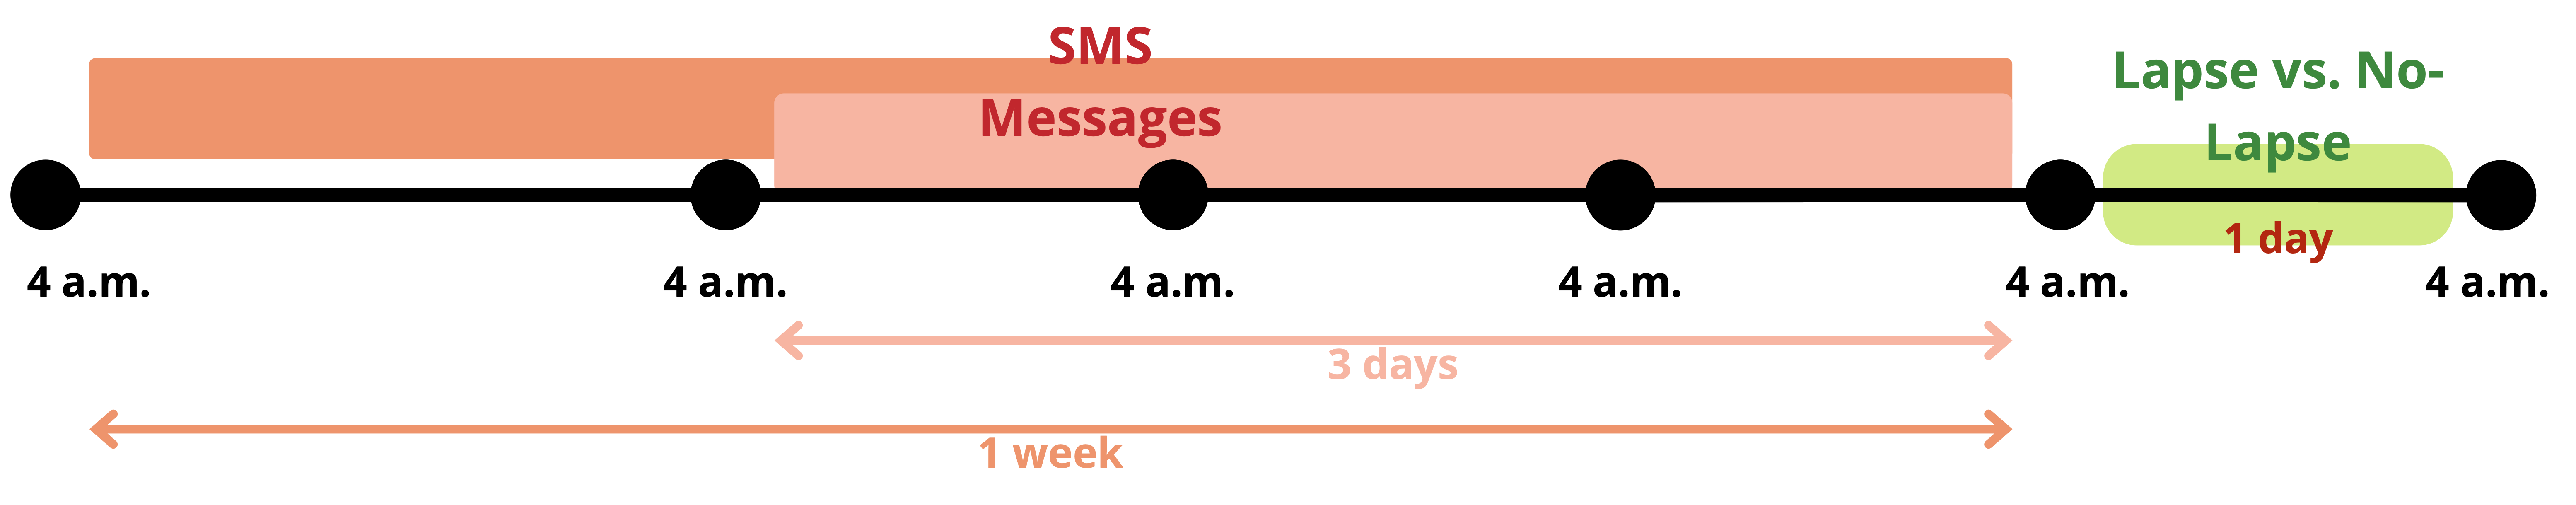
\includegraphics{images/prediction_window.png}

}

\caption{\label{fig-window}Prediction Window}

\end{figure}%

\subsection{Model Training}\label{model-training}

\subsubsection{Feature Engineering}\label{feature-engineering}

Text messages served as the only raw source for all feature engineering.
The document sets (varying based on unit of analysis) went through a
generic pre-processing step that involves removal of all emojis. Our
decision to remove all emojis was due to loss of emoji data in the ios
devices during back up. This study used the LIWC dictionary (Pennebaker
et al., 2015) and computed scores by counting frequency of words that
belong to each category. We did not remove any stop words. LIWC aligns
with the current alcohol relapse risk factor literature in that it
examines psychometric properties including cognitive state and social
processes (Brown et al., 1989; McKay, 1999, 1999).

We adopted two configurations for analytic units -- individual messages
and concatenated messages. In the first configuration method, we ran
individual messages within the defined prediction window through LIWC.
We then normalized LIWC feature scores based on the square root of word
counts instead of raw word counts which was the default choice from the
program. We applied the normalization on all LIWC categories other than
word count, word per sentence, and the four summary measures --
analytic, clout, authenticity, and tone. We excluded the four summary
categories because their raw scores were not normalized on raw word
counts. Our normalization method was chosen due to the relatively short
message length for individual messages. We further obtained the median
and 95\% percentile of normalized LIWC scores for all messages related
to each lapse label.

In the other analytic unit configuration, we first concatenated all
messages associated with each lapse label altogether. We then obtained
LIWC results for the concatenated messages. We further adopted three
configurations for normalization methods -- normalized on raw word count
(i.e., default method from the program), normalized on the square root
of word count, and a combination of these two.

\subsubsection{Candidate Algorithm}\label{candidate-algorithm}

We leveraged the XGBoost algorithm that differed on the above three
configurations: 1) prediction window length (see \emph{Section SMS
Messages}); 2) analytic units (see \emph{Section Feature Engineering});
and 3) normalization methods (see \emph{Section Feature Engineering}).
As we have a fairly imbalanced class labels in our dataset (see
\emph{Section Sample Distribution}), we further considered different
resampling strategies including upsampling and downsampling with
different ratios. Our decision to use the XGBoost algorithm was based on
its two benefits. First, the algorithm has demonstrated satisfying
performance in classifying lapse vs.~no lapse in our lab's previous work
(Wyant et al., 2024). We can select the best model from a range of
model-specific hyperparameters (mtry, tree depth, and learning rate), on
top of the four above manually incorporated configurations. Second,
XGBoost is well-suited to calculate Shapley values that can help us
understand each feature's contributions to model output (see
\emph{Section Feature Importance}).

\subsubsection{Model Selection}\label{model-selection}

We performed grouped, nested cross-validations to perform hyperparameter
tuning and select the best model configuration. The dataset was
participant-grouped so that each individual was assigned to either
held-in or held-out set to avoid bias of predicting participants' lapses
using their own data. The nested cross-validation method uses two nested
loops to divide folds. In the inner loop, held-out folds were used as a
validation set for model selection. In the outer loop, held-out folds
were utilized as a test set for model evaluation. We only presented
validation results from the 300 sets in the inner loop in this paper
because we are still working on model development. We reserved test set
to evaluate the overfitting of final full model.

The primary performance metric to select the best model configuration
and evaluate the model performance on the test sets was auROC. The auROC
measures the probability that a randomly chosen positive case is
assigned a higher score than a randomly chosen negative case. It
reflects the model's ability to distinguish between the positive and
negative cases across all possible thresholds. Values between .70 and
.80 are considered fair, values between .80 and .90 are considered good,
and values above .90 are considered excellent. Across all models that
differed on the above discussed configurations, the best model was
selected based on the highest median auROC across all validation sets
(see \emph{Section Machine Learning Algorithm}).

\subsection{Model Evaluation}\label{model-evaluation}

\subsubsection{Performance Evaluation}\label{performance-evaluation}

We calculated the predicted probability scores for all our observations
based on the best model configuration and then obtained the median auROC
score across all 300 validation sets in the inner fold. We further
performed a Bayesian hierarchical generalized linear model to estimate
the posterior probability (i.e., the likelihood of achieving the results
given out data) distributions of the auROCs. The two random intercepts
in the models included the repeat and the fold within repeat. We
reported the 95\% CIs for our models' auROCs and determined if they
included .5 (chance performance). If this CI included 0.5, we would
conclude that our model performed no better than random guess. We also
reported the probability that the model auROC is \textgreater.05.

\subsubsection{Algorithmic Bias}\label{algorithmic-bias}

A subset of individual characteristic measures was used to evaluate
model fairness on subgroups. We compared model performance among each
sex, racial, age and income subgroups because the populations face
increased barriers obtaining AUD treatments. Stigma among older
populations and wome, and economic hardship in racial minority groups
can all contribute to low treatment-seeking and alcohol treatment
completion (DiBartolo \& Jarosinski, 2017; J. O. Jacobson et al., 2007;
May et al., 2019). Participants younger than 55 years old were
considered as a privileged group. We adopted half of median income in
Madison area in 2017 as cut-off to assign participants to income groups.

We performed a Bayesian hierarchical generalized linear model that
regressed the auROCs from the 300 validation sets in the inner loop as a
function of group membership (privileged group vs.~unprivileged group
within each of above individual characteristics). We reported the 95\%
CI for model performance differences and examined if they included 0. If
this CI did not include 0, we would conclude that our model was unfair.
We also reported the probability that the difference is greater than
zero.

\subsubsection{Feature Importance}\label{feature-importance}

We also calculated SHAP values to interpret the results. SHAP is a game
theory based method to explain how each feature influences the model
output (Lundberg \& Lee, 2017). It assigns importance to each feature,
where a positive feature importance positively affects the model output.
This methodology can be applied to any machine learning algorithm and
can increase model transparency and interpretability. Local Shapley
values explain factors that contribute to a single observation, and
global Shapley values represent feature importance across all
observations. To compute global Shapley values, we averaged the absolute
value of all local Shapley values. For better understanding, we
aggregated Shapley values for each LIWC category, regardless of their
prediction window and normalization methods.

\newpage

\section{Results}\label{results}

\subsection{Demographics}\label{demographics}

The final sample includes 138 participants. On average, participants are
39.60 years old (SD = 11.17, range = 21-66). 65 (47.10\%) participants
are females, 121 (87.68\%) are White/Caucasian, 3 (2.17\%) are American
Indiain/Alaska Native, 2 (1.45\%) are Asian, 6 (4.35\%) are
Black/African American, and 6 (4.35\%) are Other/Multiracial. See
Table~\ref{tbl-demographics} for more details on participant
demographics (education, employment, income, marital status) and their
patterns of alcohol use.

\begin{longtable}[]{@{}
  >{\raggedright\arraybackslash}p{(\columnwidth - 10\tabcolsep) * \real{0.7753}}
  >{\centering\arraybackslash}p{(\columnwidth - 10\tabcolsep) * \real{0.0449}}
  >{\centering\arraybackslash}p{(\columnwidth - 10\tabcolsep) * \real{0.0449}}
  >{\centering\arraybackslash}p{(\columnwidth - 10\tabcolsep) * \real{0.0449}}
  >{\centering\arraybackslash}p{(\columnwidth - 10\tabcolsep) * \real{0.0449}}
  >{\centering\arraybackslash}p{(\columnwidth - 10\tabcolsep) * \real{0.0449}}@{}}
\toprule\noalign{}
\begin{minipage}[b]{\linewidth}\raggedright
\end{minipage} & \begin{minipage}[b]{\linewidth}\centering
N
\end{minipage} & \begin{minipage}[b]{\linewidth}\centering
\%
\end{minipage} & \begin{minipage}[b]{\linewidth}\centering
M
\end{minipage} & \begin{minipage}[b]{\linewidth}\centering
SD
\end{minipage} & \begin{minipage}[b]{\linewidth}\centering
Range
\end{minipage} \\
\midrule\noalign{}
\endfirsthead
\toprule\noalign{}
\begin{minipage}[b]{\linewidth}\raggedright
\end{minipage} & \begin{minipage}[b]{\linewidth}\centering
N
\end{minipage} & \begin{minipage}[b]{\linewidth}\centering
\%
\end{minipage} & \begin{minipage}[b]{\linewidth}\centering
M
\end{minipage} & \begin{minipage}[b]{\linewidth}\centering
SD
\end{minipage} & \begin{minipage}[b]{\linewidth}\centering
Range
\end{minipage} \\
\midrule\noalign{}
\endhead
\bottomrule\noalign{}
\endlastfoot
\textbf{Age} & --- & --- & 39.60 & 11.17 & 21-66 \\
\textbf{Sex} & & & & & \\
\emph{Female} & 73 & 52.90\% & --- & --- & --- \\
\emph{Male} & 65 & 47.10\% & --- & --- & --- \\
\textbf{Race} & & & & & \\
\emph{White/Caucasian} & 121 & 87.68\% & --- & --- & --- \\
\emph{American Indian/Alaska Native} & 3 & 2.17\% & --- & --- & --- \\
\emph{Asian} & 2 & 1.45\% & --- & --- & --- \\
\emph{Black/African American} & 6 & 4.35\% & --- & --- & --- \\
\emph{Other/Multiracial} & 6 & 4.35\% & --- & --- & --- \\
\textbf{Ethnicity} & & & & & \\
\emph{Mexican, Mexican American, Chicano} & 3 & 2.17\% & --- & --- &
--- \\
\emph{Another Hispanic, Latino, or Spanish Origin} & 1 & 0.72\% & --- &
--- & --- \\
\emph{Not Hispanic, Latino, or Spanish Origin} & 134 & 97.10\% & --- &
--- & --- \\
\textbf{Highest Education} & & & & & \\
\emph{2-Year degree} & 13 & 9.42\% & --- & --- & --- \\
\emph{Advanced degree} & 23 & 16.67\% & --- & --- & --- \\
\emph{College degree} & 54 & 39.13\% & --- & --- & --- \\
\emph{High school or GED} & 11 & 7.97\% & --- & --- & --- \\
\emph{Less than high school or GED degree} & 1 & 0.72\% & --- & --- &
--- \\
\emph{Some college} & 36 & 26.09\% & --- & --- & --- \\
\textbf{Employment} & & & & & \\
\emph{Disabled} & 4 & 2.90\% & --- & --- & --- \\
\emph{Employed} & 96 & 69.57\% & --- & --- & --- \\
\emph{Full-time student} & 7 & 5.07\% & --- & --- & --- \\
\emph{Homemaker} & 1 & 0.72\% & --- & --- & --- \\
\emph{Other, not otherwise specified} & 8 & 5.80\% & --- & --- & --- \\
\emph{Retired} & 6 & 4.35\% & --- & --- & --- \\
\emph{Temporarily laid off, sick leave, or maternity leave} & 3 & 2.17\%
& --- & --- & --- \\
\emph{Unemployed} & 13 & 9.42\% & --- & --- & --- \\
\textbf{Total Personal Gross Income} & --- & --- & 36,494.41 & 32,149.41
& 0-200,000 \\
\textbf{Marital Status} & & & & & \\
\emph{Divorced} & 40 & 29.90\% & --- & --- & --- \\
\emph{Married} & 30 & 21.74\% & --- & --- & --- \\
\emph{Never Married} & 61 & 44.20\% & --- & --- & --- \\
\emph{Separated} & 5 & 3.62\% & --- & --- & --- \\
\emph{Widowed} & 2 & 1.45\% & --- & --- & --- \\
\textbf{Alcohol Use History} & & & & & \\
\emph{Age of First Drink Without Family} & --- & --- & 14.62 & 2.98 &
6-24 \\
\emph{Age of First Regular Drink} & --- & --- & 19.39 & 6.05 & 11-53 \\
\emph{Age of First Drinking Problem} & --- & --- & 27.62 & 9.42 &
15-60 \\
\emph{Age of First Quit Attempt} & --- & --- & 31.02 & 10.09 & 15-61 \\
\emph{Number of Quit Attempts} & --- & --- & 5.98 & 9.83 & 0-100 \\
\emph{Types of Programs or Services Used} & & & & & \\
\emph{Long-Term Residential Treatment (more than 6 months)} & 6 & 4.35\%
& --- & --- & --- \\
\emph{Short-Term Residential Treatment (less than 6 months)} & 41 &
29.71\% & --- & --- & --- \\
\emph{Outpatient Treatment} & 64 & 46.38\% & --- & --- & --- \\
\emph{Individual Counseling} & 91 & 65.94\% & --- & --- & --- \\
\emph{Group Counseling} & 57 & 41.30\% & --- & --- & --- \\
\emph{Alcoholics Anonymous/Narcotics Anonymous} & 84 & 60.87\% & --- &
--- & --- \\
\emph{Other} & 38 & 27.54\% & --- & --- & --- \\
\emph{Even Taken Prescribed Medication} & 53 & 38.41\% & --- & --- &
--- \\
\emph{Number of Days per Week Consumed Any Alcohol} & --- & --- & 5.24 &
1.81 & 1-7 \\
\emph{Number of Days per Week Consumed 6 or More Alcoholic Drinks in One
Day} & --- & --- & 3.94 & 2.07 & 0-7 \\
\emph{Number of Alcoholic Drinks per Day on Days Drinked} & --- & --- &
7.43 & 4.31 & 1-25 \\
\textbf{DSM-5 Symptom Count} & --- & --- & 8.89 & 1.84 & 4-11 \\
\textbf{Young Adult Alcohol Problems Test} & --- & --- & 19.90 & 4.60 &
6-27 \\
\textbf{Past 3-Month Drug Use (WHO-The Alcohol, Smoking and Substance
Involvement Screening Test)} & & & & & \\
\emph{Tobacco products (cigarettes, chewing tobacco, cigars, etc.)} & 75
& 54.35\% & --- & --- & --- \\
\emph{Cannabis (marijuana, pot, grass, hash, etc.)} & 64 & 46.38\% & ---
& --- & --- \\
\emph{Cocaine (coke, crack, etc.)} & 17 & 12.32\% & --- & --- & --- \\
\emph{Amphetamine type stimulants (speed, diet pills, ecstasy, etc.)} &
15 & 10.87\% & --- & --- & --- \\
\emph{Inhalants (nitrous, glue, petrol, paint thinner, etc.)} & 3 &
2.17\% & --- & --- & --- \\
\emph{Sedatives or Sleeping Pills (Valium, Serepax, Rohypnol, etc.)} &
21 & 15.22\% & --- & --- & --- \\
\emph{Hallucinogens (LSD, acid, mushrooms, PCP, Special K, etc.)} & 14 &
10.14\% & --- & --- & --- \\
\emph{Opioids (heroin, morphine, methadone, codeine, etc.)} & 14 &
10.14\% & --- & --- & --- \\
\caption{Participant demographics and alcohol use
history}\label{tbl-demographics}\tabularnewline
\end{longtable}

\subsection{Sample Distribution}\label{sample-distribution}

The final total number of lapse labels in the dataset is 11562. 7.63\%
of the labels are associated with a lapse episode. On average, each
participant has 83.78 labels (sd = 11.35, median = 88.00, range = 30 -
90; see Figure~\ref{fig-lapse_count}).

\begin{figure}[H]

\centering{

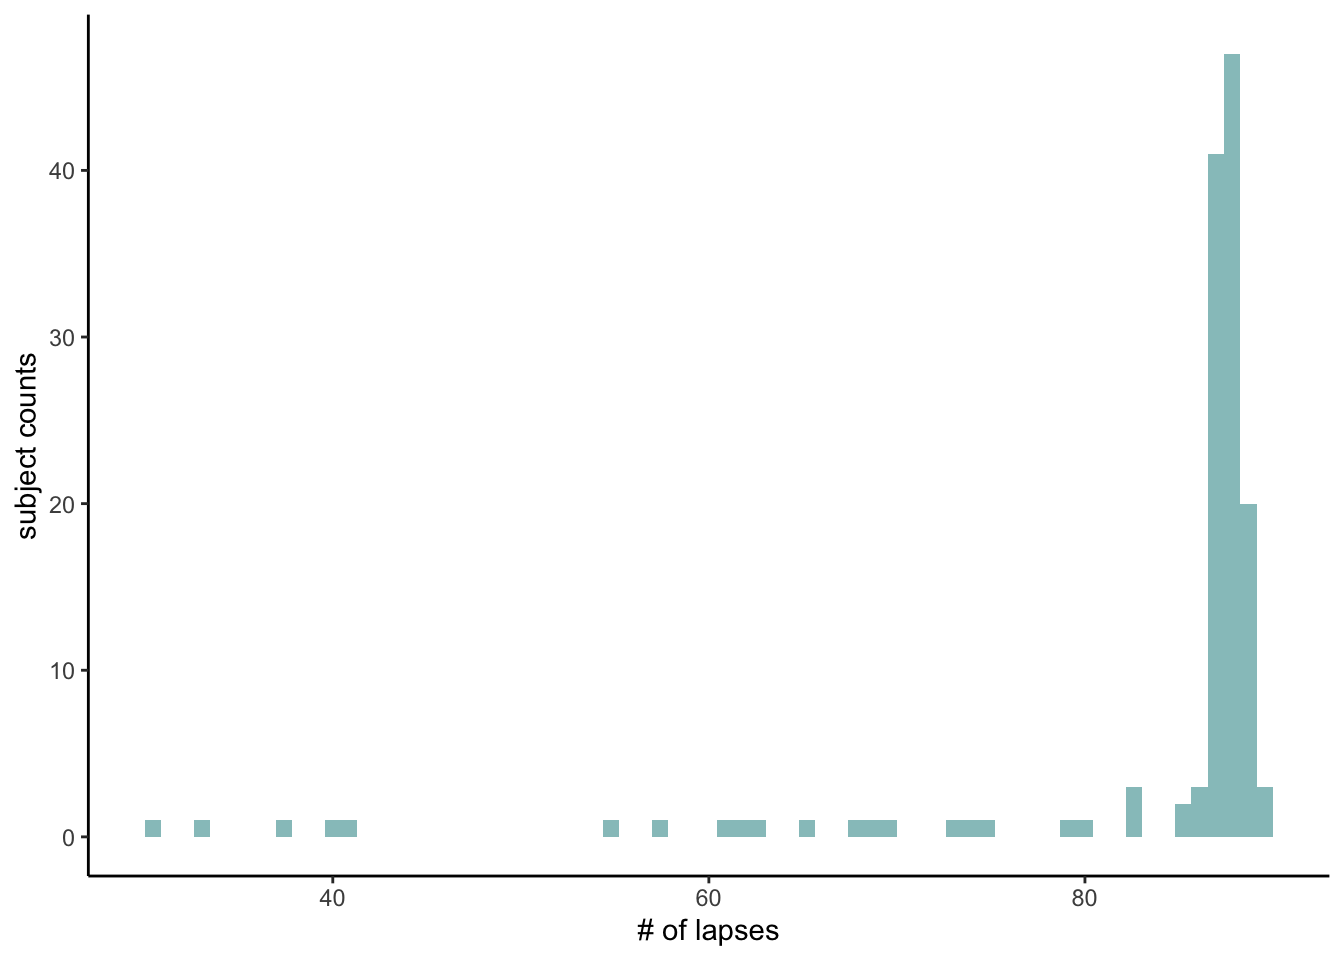
\includegraphics{index_files/figure-latex/notebooks-fig_eda_messages-fig-lapse_count-output-1.png}

}

\caption{\label{fig-lapse_count}Distribution of Lapse Label Counts}

\end{figure}%

\textsubscript{Source:
\href{https://jjcurtin.github.io/study_messages/notebooks/fig_eda_messages-preview.html\#cell-fig-lapse_count}{EDA
on Raw Messages}}

The total number of messages in the dataset is 313492. On average, each
subject has 2271.68 messages (sd = 2536.60, range = 100 - 15884). The
average message length across all participants is 10.42 words (sd =
14.30, median = 7.00, range = 1 - 1266). On average, each participant
has a mean message length of 10.87 (sd = 3.97, range = 5.25 - 38.91).

\begin{figure}[H]

\centering{

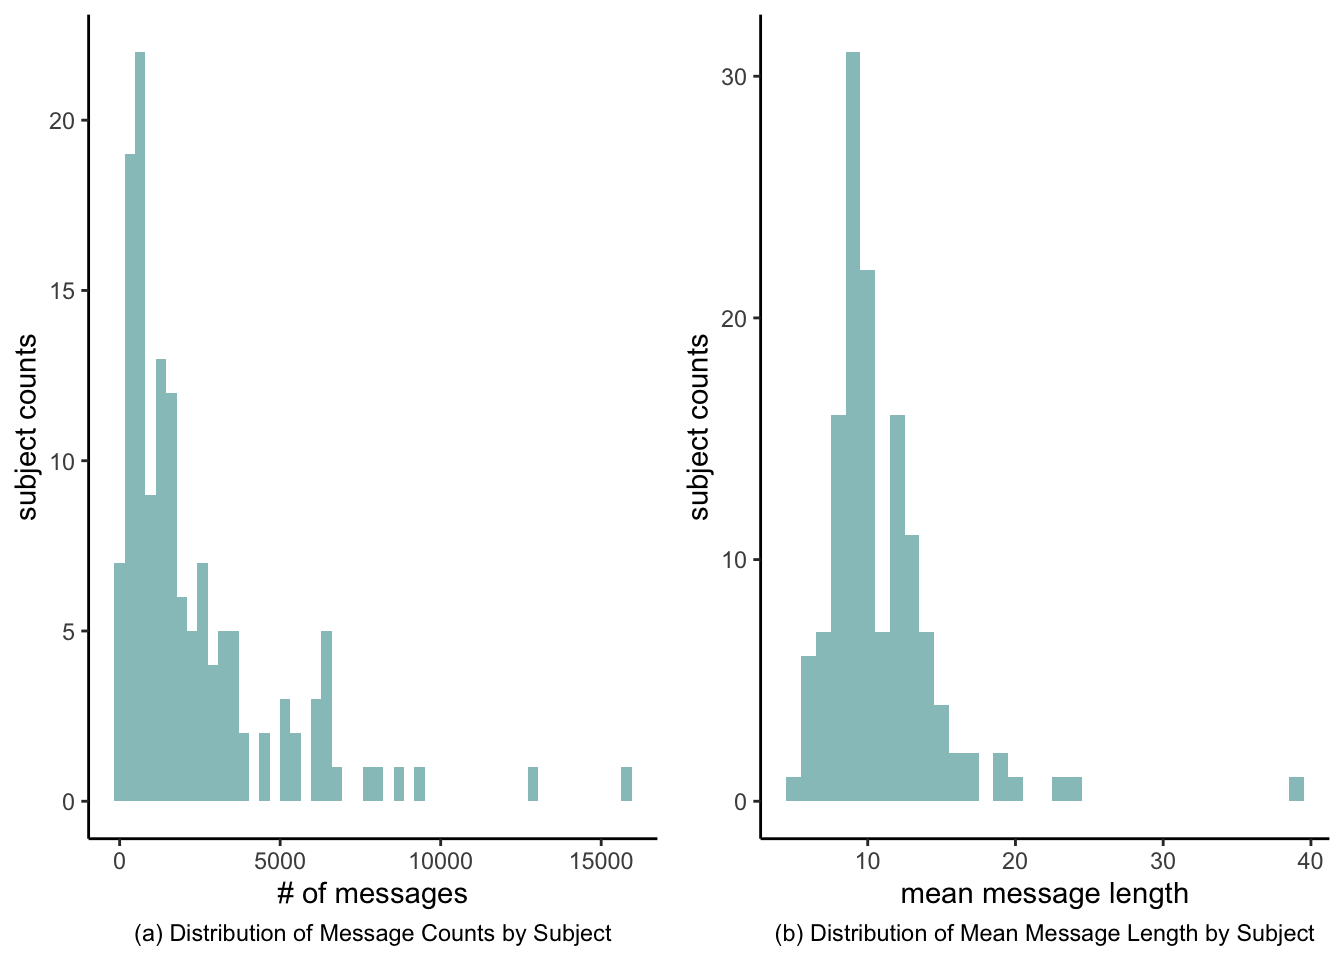
\includegraphics{index_files/figure-latex/notebooks-fig_eda_messages-fig-raw-output-1.png}

}

\caption{\label{fig-raw}Sample Characteristics of Raw Messages}

\end{figure}%

\textsubscript{Source:
\href{https://jjcurtin.github.io/study_messages/notebooks/fig_eda_messages-preview.html\#cell-fig-raw}{EDA
on Raw Messages}}

On average, each lapse label has 79.21 messages (sd = 112.13, median =
40.00, range = 1 - 1414) during the 3-day prediction window. 11.92\% of
labels have no associated messages in the previous 3 days. Each
participant has an averaged 79.48 messages as predictors per label (sd =
87.12, median = 50.12, range = 2.97 - 529.45). On average, each
participant's data missingness is 12.28\% (sd = 19.42\%, median =
1.14\%, range = 0.00\% - 77.27\%).

\begin{figure}[H]

\centering{

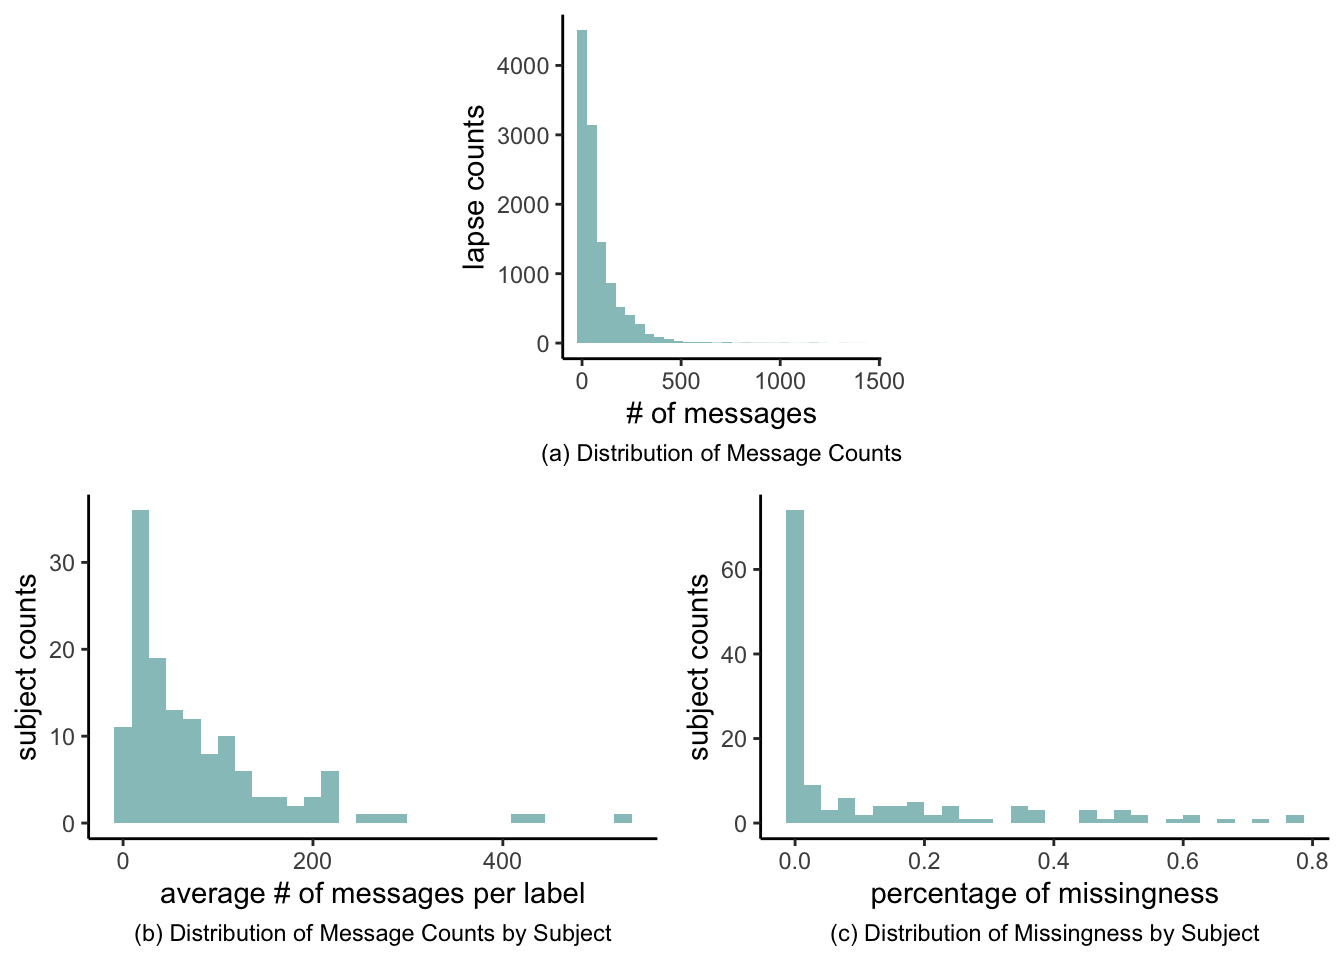
\includegraphics{index_files/figure-latex/notebooks-fig_eda_messages-fig-3day-output-2.png}

}

\caption{\label{fig-3day}Sample Characteristics in the 3-Day Prediction
Window}

\end{figure}%

\textsubscript{Source:
\href{https://jjcurtin.github.io/study_messages/notebooks/fig_eda_messages-preview.html\#cell-fig-3day}{EDA
on Raw Messages}}

On average, each lapse label has 180.42 messages (sd = 241.30, median =
96.00, range = 1 - 2866) during the 1-week prediction window. 7.83\% of
labels have no associated messages in the previous week. Each
participant has an averaged 181.23 messages as predictors per label (sd
= 199.32, median = 113.47, range = 6.75 - 1200.76). On average, each
participant's data missingness is 8.14\% (sd = 16.23\%, median = 0.00\%,
range = 0.00\% - 72.73\%).

\begin{figure}[H]

\centering{

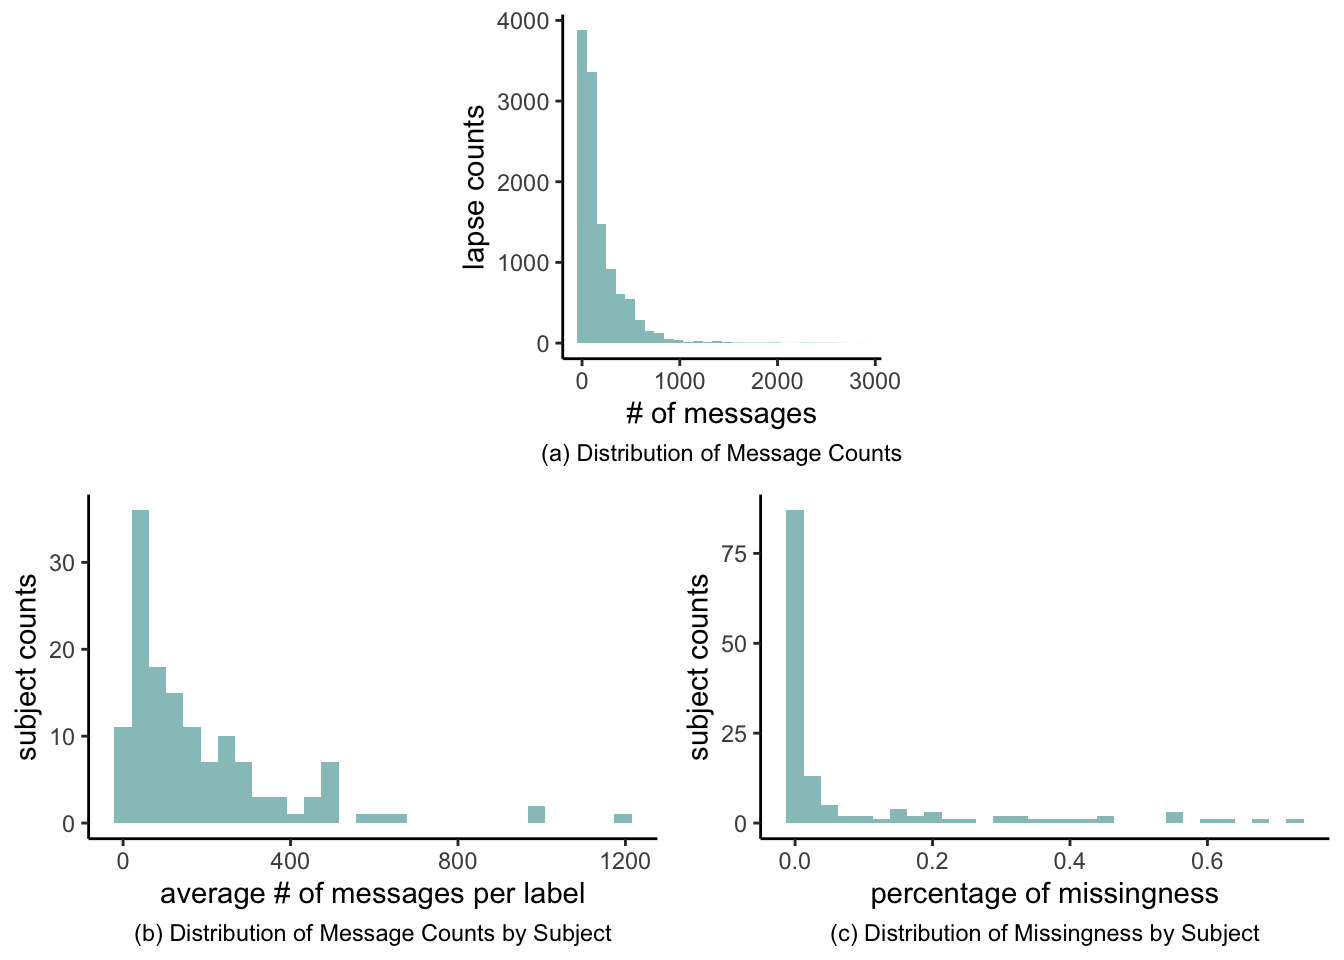
\includegraphics{index_files/figure-latex/notebooks-fig_eda_messages-fig-1week-output-2.png}

}

\caption{\label{fig-1week}Sample Characteristics in the 1-Week
Prediction Window}

\end{figure}%

\textsubscript{Source:
\href{https://jjcurtin.github.io/study_messages/notebooks/fig_eda_messages-preview.html\#cell-fig-1week}{EDA
on Raw Messages}}

\subsection{LIWC Features}\label{liwc-features}

We obtained LIWC scores from 117 linguistic categories. These categories
include total word count, number of words per sentence, the four summary
categories (analytic, clout, authentic, and tone), and other linguistic
categories such as social and pronouns. Notably, LIWC-22 now
incorporates a \emph{health} dimension that includes phrases related to
illness, wellness, mental health (diagnoses or behaviors), and
substances. For each unit of analysis, we had 468 engineered features
after normalization and aggregation (see \emph{Section Feature
Engineering}).

When our unit of analysis was on individual messages (see
Table~\ref{tbl-panel} and Figure~\ref{fig-liwc_ind}), the median of all
median LIWC feature scores excluding the six unnormalized categories
within each 3-day prediction window ranged from 0.00 to 2.45 (median =
0.00, sd = 0.34). The median of all median LIWC feature scores excluding
the six unnormalized categories within each 1-week prediction window
ranged from 0.00 to 2.45 (median = 0.00, sd = 0.35). The max of all
median LIWC feature scores excluding the six unnormalized categories
within each 3-day prediction window ranged from 0.00 to 11.58 (median =
0.80, sd = 1.60). The max of all median LIWC feature scores excluding
the six unnormalized categories within each 1-week prediction window
ranged from 0.00 to 8.89 (median = 0.63, sd = 1.25).

The median of all 95\% percentile LIWC feature scores excluding the six
unnormalized categories within each 3-day prediction window ranged from
0.00 to 4.74 (median = 0.30, sd = 0.70). The median of all 95\%
percentile LIWC feature scores excluding the six unnormalized categories
within each 1-week prediction window ranged from 0.00 to 4.89 (median =
0.34, sd = 0.72). The max of all 95\% percentile LIWC feature scores
excluding the six unnormalized categories within each 3-day prediction
window ranged from 0.36 to 17.51 (median = 1.15, sd = 2.40). The max of
all 95\% percentile LIWC feature scores excluding the six unnormalized
categories within each 1-week prediction window ranged from 0.35 to
18.42 (median = 1.00, sd = 2.47).

\begin{table}

\begin{minipage}{\linewidth}

\centering{

\begin{tabular}{lllll}
\toprule
 & SD & Median & Min & Max\\
\midrule
wc\_median & 5.43 & 7.00 & 1.00 & 142.00\\
wc\_q\_95 & 20.31 & 26.40 & 1.00 & 369.05\\
wps\_median & 2.45 & 5.00 & 0.00 & 78.00\\
wps\_q\_95 & 5.96 & 14.75 & 0.00 & 78.00\\
analytic\_median & 17.11 & 10.19 & 1.00 & 99.00\\
analytic\_q\_95 & 19.24 & 97.20 & 1.00 & 99.00\\
clout\_median & 32.72 & 40.06 & 1.00 & 99.00\\
clout\_q\_95 & 12.98 & 99.00 & 1.00 & 99.00\\
authentic\_median & 19.60 & 89.39 & 1.00 & 99.00\\
authentic\_q\_95 & 10.77 & 99.00 & 1.00 & 99.00\\
tone\_median & 17.84 & 99.00 & 1.00 & 99.00\\
tone\_q\_95 & 9.85 & 99.00 & 1.00 & 99.00\\
\bottomrule
\end{tabular}

}

\subcaption{\label{tbl-ind_3day}3-Day Prediction Window}

\end{minipage}%
\newline
\begin{minipage}{\linewidth}

\centering{

\begin{tabular}{lllll}
\toprule
 & SD & Median & Min & Max\\
\midrule
wc\_median & 4.00 & 7.00 & 1.00 & 81.00\\
wc\_q\_95 & 17.84 & 28.00 & 1.00 & 404.00\\
wps\_median & 2.20 & 5.00 & 1.00 & 78.00\\
wps\_q\_95 & 5.53 & 15.10 & 1.00 & 78.00\\
analytic\_median & 14.02 & 10.19 & 1.00 & 99.00\\
analytic\_q\_95 & 14.85 & 98.59 & 1.00 & 99.00\\
clout\_median & 30.57 & 40.06 & 1.00 & 99.00\\
clout\_q\_95 & 9.94 & 99.00 & 1.00 & 99.00\\
authentic\_median & 15.87 & 89.39 & 1.00 & 99.00\\
authentic\_q\_95 & 7.36 & 99.00 & 1.00 & 99.00\\
tone\_median & 13.85 & 99.00 & 1.00 & 99.00\\
tone\_q\_95 & 7.27 & 99.00 & 1.00 & 99.00\\
\bottomrule
\end{tabular}

}

\subcaption{\label{tbl-ind_1week}1-Week Prediction Window}

\end{minipage}%

\caption{\label{tbl-panel}Sample Characteristics of Engineered Feature
Scores (Median and 95\% Quantile Scores from Individual Messages) for
the Six Unnormalized Categories Within Each Prediction Window}

\end{table}%

\begin{figure}[H]

\centering{

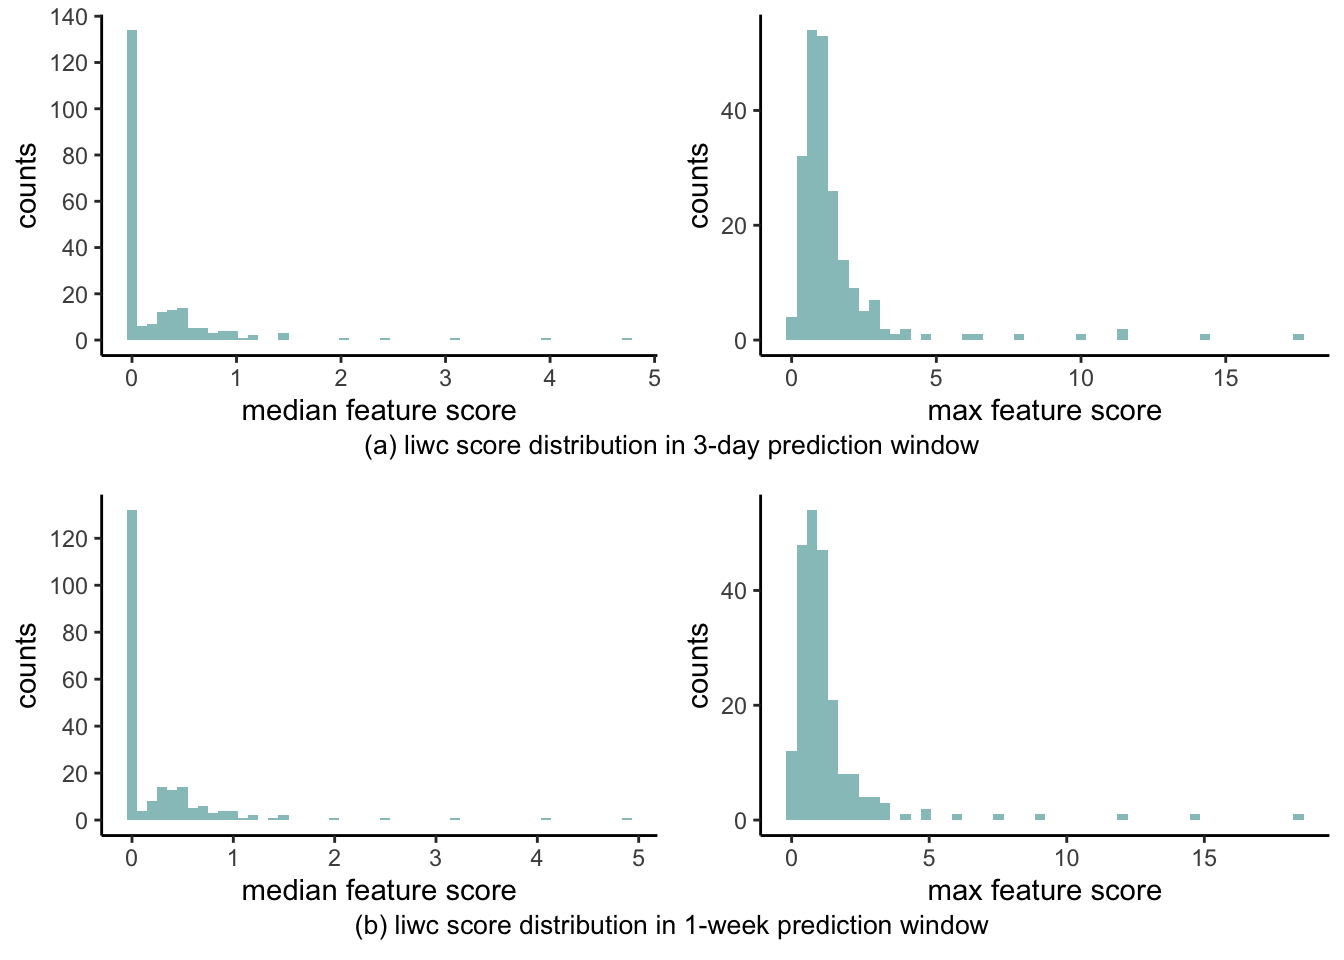
\includegraphics{index_files/figure-latex/notebooks-fig_eda_liwc-fig-liwc_ind-output-1.png}

}

\caption{\label{fig-liwc_ind}Distribution of Engineered Feature Scores
(Median or 95\% Percentile of Normalized LIWC Score From Individual
Messages) Within Each Prediction Window}

\end{figure}%

\textsubscript{Source:
\href{https://jjcurtin.github.io/study_messages/notebooks/fig_eda_liwc-preview.html\#cell-fig-liwc_ind}{EDA
on LIWC Features}}

When our unit of analysis was on concatenated messages (see
Table~\ref{tbl-panel2}, Figure~\ref{fig-liwc_cat_raw} and
Figure~\ref{fig-liwc_cat_norm}), the median of all raw feature scores
within the 3-day prediction window ranged from 0.00 to 91.36 (median =
1.32, sd = 12.64). The median of all raw feature scores within the
1-week prediction window ranged from 0.00 to 91.30 (median = 1.36, sd =
12.63). The max of all raw feature scores within the 3-day prediction
window ranged from 3.85 to 166.67 (median = 33.33, sd = 37.64). The max
of all raw feature scores within the 1-week prediction window ranged
from 1.82 to 166.67 (median = 27.27, sd = 35.21).

The median of all normalized feature scores within the 3-day prediction
window ranged from 0.00 to 20.63 (median = 0.32, sd = 2.85). The median
of all normalized feature scores within the 1-week prediction window
ranged from 0.00 to 30.69 (median = 0.47, sd = 4.25). The max of all
normalized feature scores within the 3-day prediction window ranged from
0.37 to 106.55 (median = 2.95, sd = 15.11). The max of all normalized
feature scores within the 1-week prediction window ranged from 0.29 to
143.30 (median = 3.16, sd = 20.31).

\begin{table}

\begin{minipage}{0.50\linewidth}

\centering{

\begin{tabular}{lllll}
\toprule
 & SD & Median & Min & Max\\
\midrule
wc & 1175.22 & 512.00 & 1 & 13211\\
wps & 9.75 & 10.76 & 0 & 295\\
analytic & 16.96 & 19.05 & 1 & 99\\
clout & 25.37 & 50.20 & 1 & 99\\
authentic & 22.34 & 77.13 & 1 & 99\\
tone & 23.28 & 82.19 & 1 & 99\\
\bottomrule
\end{tabular}

}

\subcaption{\label{tbl-cat_3day}3-Day Prediction Window}

\end{minipage}%
%
\begin{minipage}{0.50\linewidth}

\centering{

\begin{tabular}{lllll}
\toprule
 & SD & Median & Min & Max\\
\midrule
wc & 2484.84 & 1124.00 & 1 & 23702\\
wps & 8.73 & 10.91 & 1 & 241\\
analytic & 14.30 & 19.17 & 1 & 99\\
clout & 22.54 & 50.15 & 1 & 99\\
authentic & 19.04 & 77.10 & 1 & 99\\
tone & 20.76 & 82.04 & 1 & 99\\
\bottomrule
\end{tabular}

}

\subcaption{\label{tbl-cat_1week}1-Week Prediction Window}

\end{minipage}%

\caption{\label{tbl-panel2}Sample Characteristics of Raw LIWC Scores on
Concatenated Messages Across the Six Linguistic Categories Within Each
Prediction Window}

\end{table}%

\begin{figure}[H]

\centering{

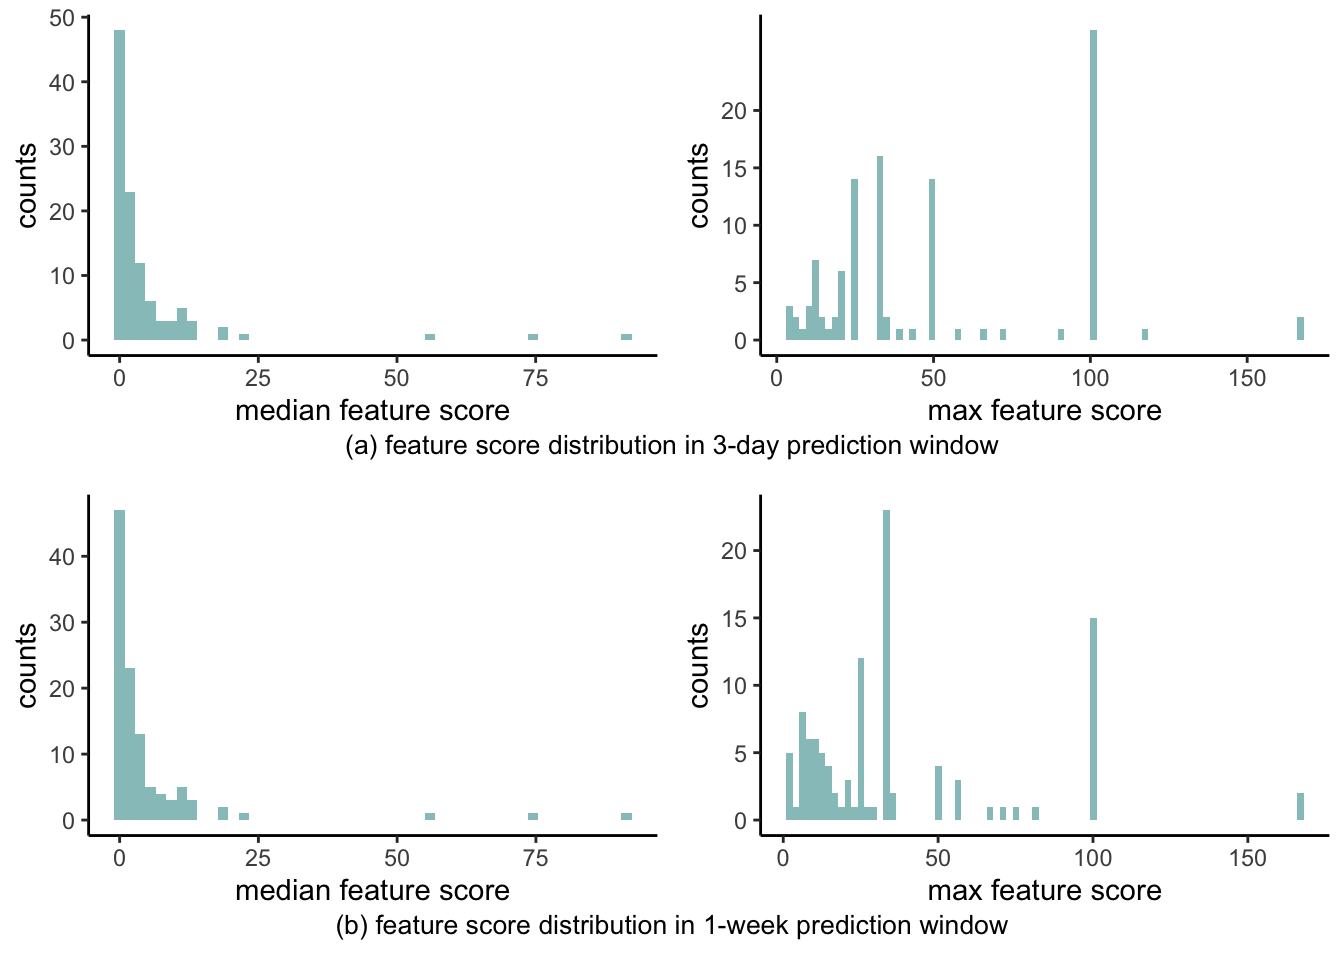
\includegraphics{index_files/figure-latex/notebooks-fig_eda_liwc-fig-liwc_cat_raw-output-1.png}

}

\caption{\label{fig-liwc_cat_raw}Distribution of Raw LIWC Feature Scores
From Concatenated Messages Within Each Prediction Window}

\end{figure}%

\textsubscript{Source:
\href{https://jjcurtin.github.io/study_messages/notebooks/fig_eda_liwc-preview.html\#cell-fig-liwc_cat_raw}{EDA
on LIWC Features}}

\begin{figure}[H]

\centering{

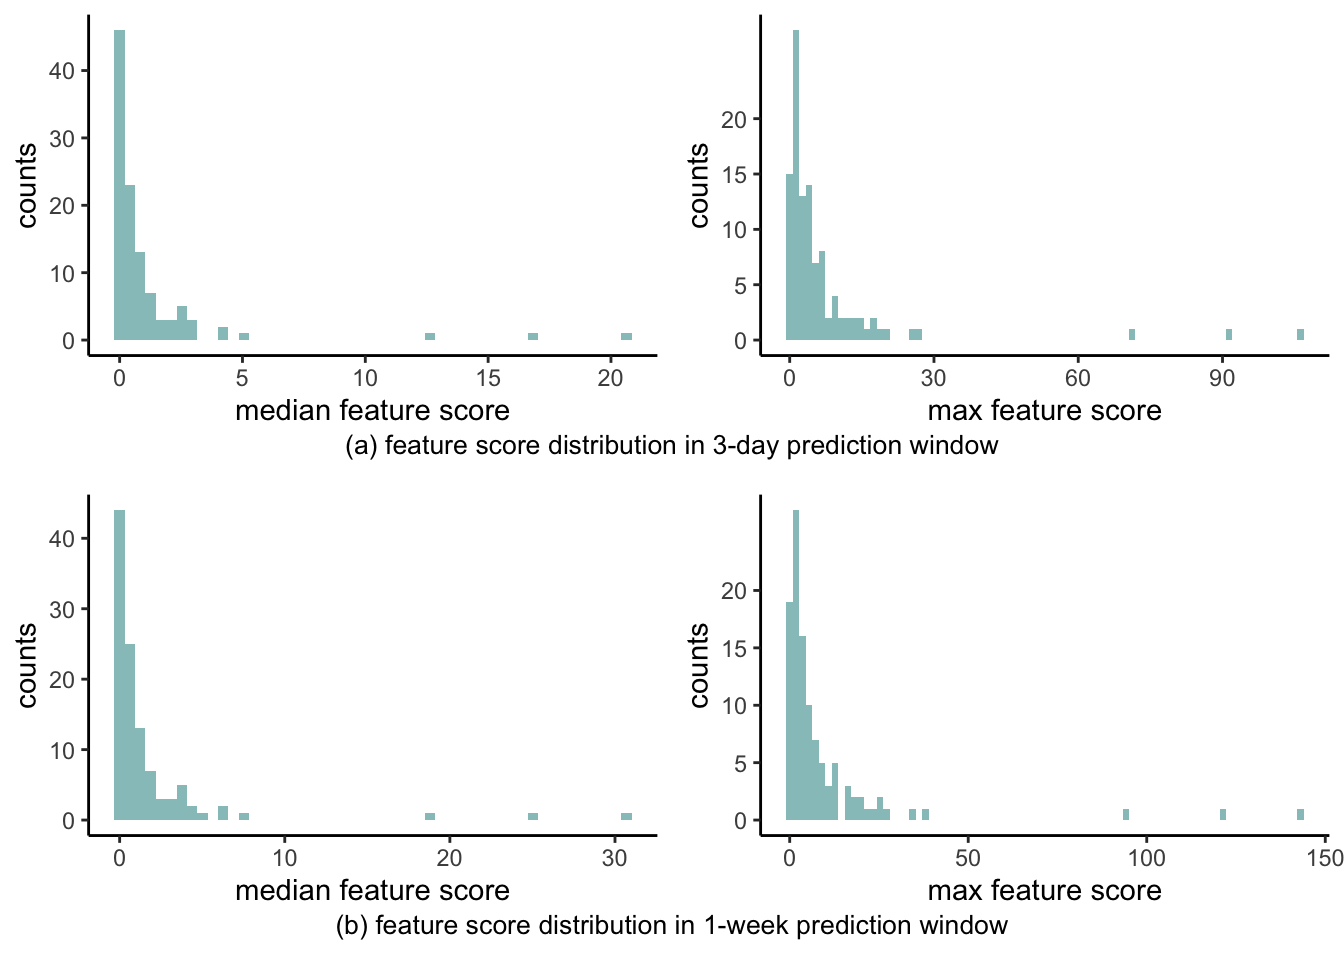
\includegraphics{index_files/figure-latex/notebooks-fig_eda_liwc-fig-liwc_cat_norm-output-1.png}

}

\caption{\label{fig-liwc_cat_norm}Distribution of Normalized LIWC
Feature Scores From Concatenated Messages Within Each Prediction Window}

\end{figure}%

\textsubscript{Source:
\href{https://jjcurtin.github.io/study_messages/notebooks/fig_eda_liwc-preview.html\#cell-fig-liwc_cat_norm}{EDA
on LIWC Features}}

\subsection{Best Model Evaluation}\label{best-model-evaluation}

The best model configuration was the one that leveraged raw LWIC scores
from concatenated messages within both the 3-day and 1-week prediction
window, and an upsampling technique with a ratio of 1:1. We applied the
best configuration on the raw dataset and obtained an auROC score of
0.53 (see Figure~\ref{fig-auroc} for the ROC curve). We further
aggregated predictions by folds, and the median score of all median
auROCs across the 300 inner folds was 0.53 (sd = 0.09, range = 0.28 -
0.80; see Figure~\ref{fig-auroc_hist}). The median posterior
distribution of the auROCs was 0.53 (95\% CI = {[}0.52, 0.54{]}; see
Figure~\ref{fig-auroc_posterior}). The probability of the posterior
auROC larger than .5 was 1.00. We concluded that our model was better
than chance performance.

\begin{figure}[H]

\centering{

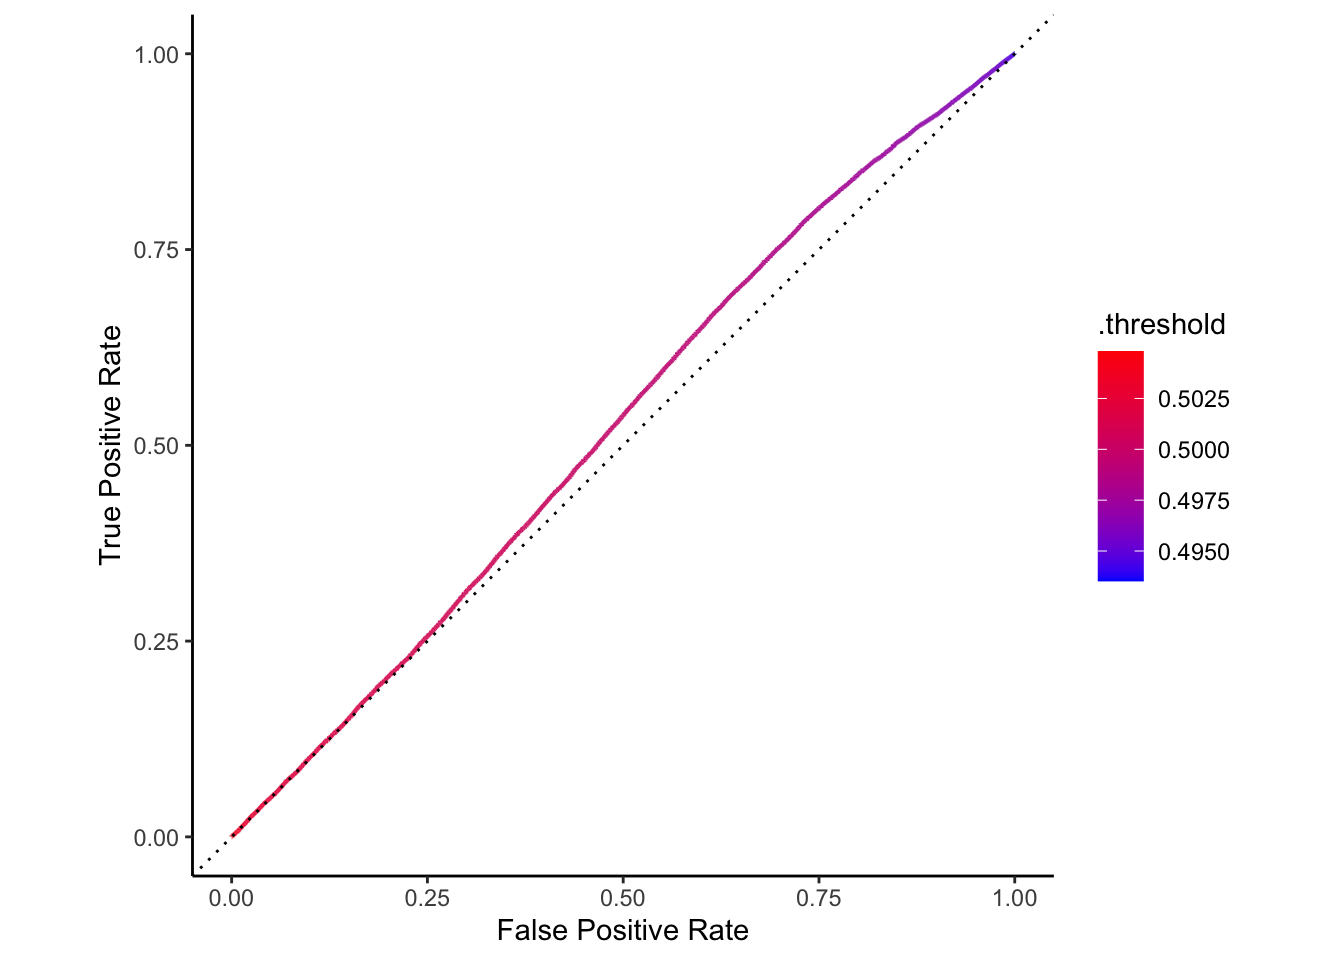
\includegraphics{index_files/figure-latex/notebooks-fig_auroc-fig-auroc-output-2.png}

}

\caption{\label{fig-auroc}ROC Curve for the Best Model Configuration}

\end{figure}%

\textsubscript{Source:
\href{https://jjcurtin.github.io/study_messages/notebooks/fig_auroc-preview.html\#cell-fig-auroc}{Performance
plots}}

\begin{figure}[H]

\centering{

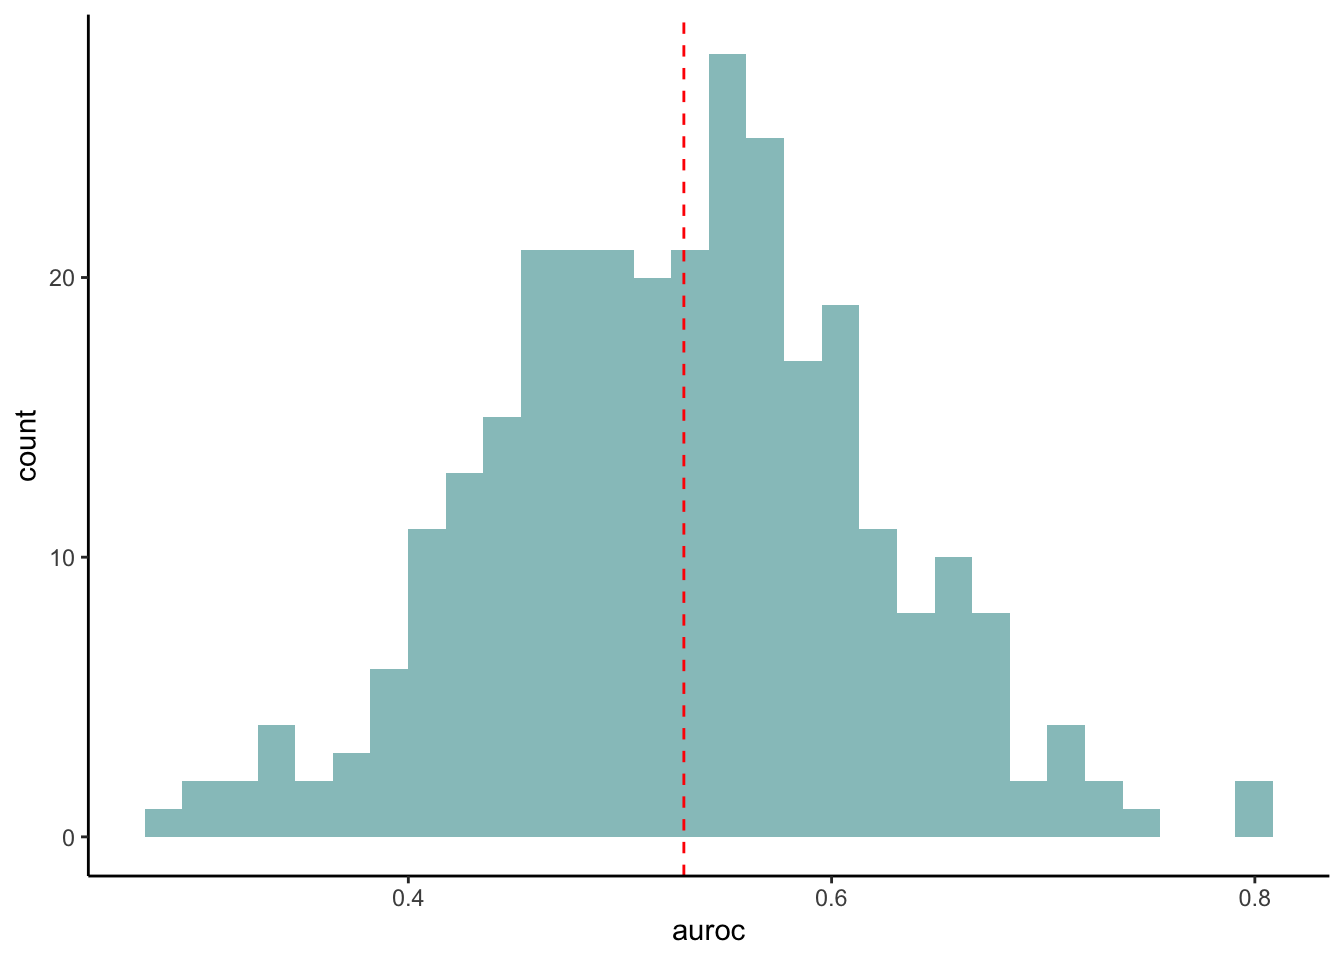
\includegraphics{index_files/figure-latex/notebooks-fig_auroc-fig-auroc_hist-output-2.png}

}

\caption{\label{fig-auroc_hist}Distribution of auROCs Across 300 Inner
Folds}

\end{figure}%

\textsubscript{Source:
\href{https://jjcurtin.github.io/study_messages/notebooks/fig_auroc-preview.html\#cell-fig-auroc_hist}{Performance
plots}}

\begin{figure}[H]

\centering{

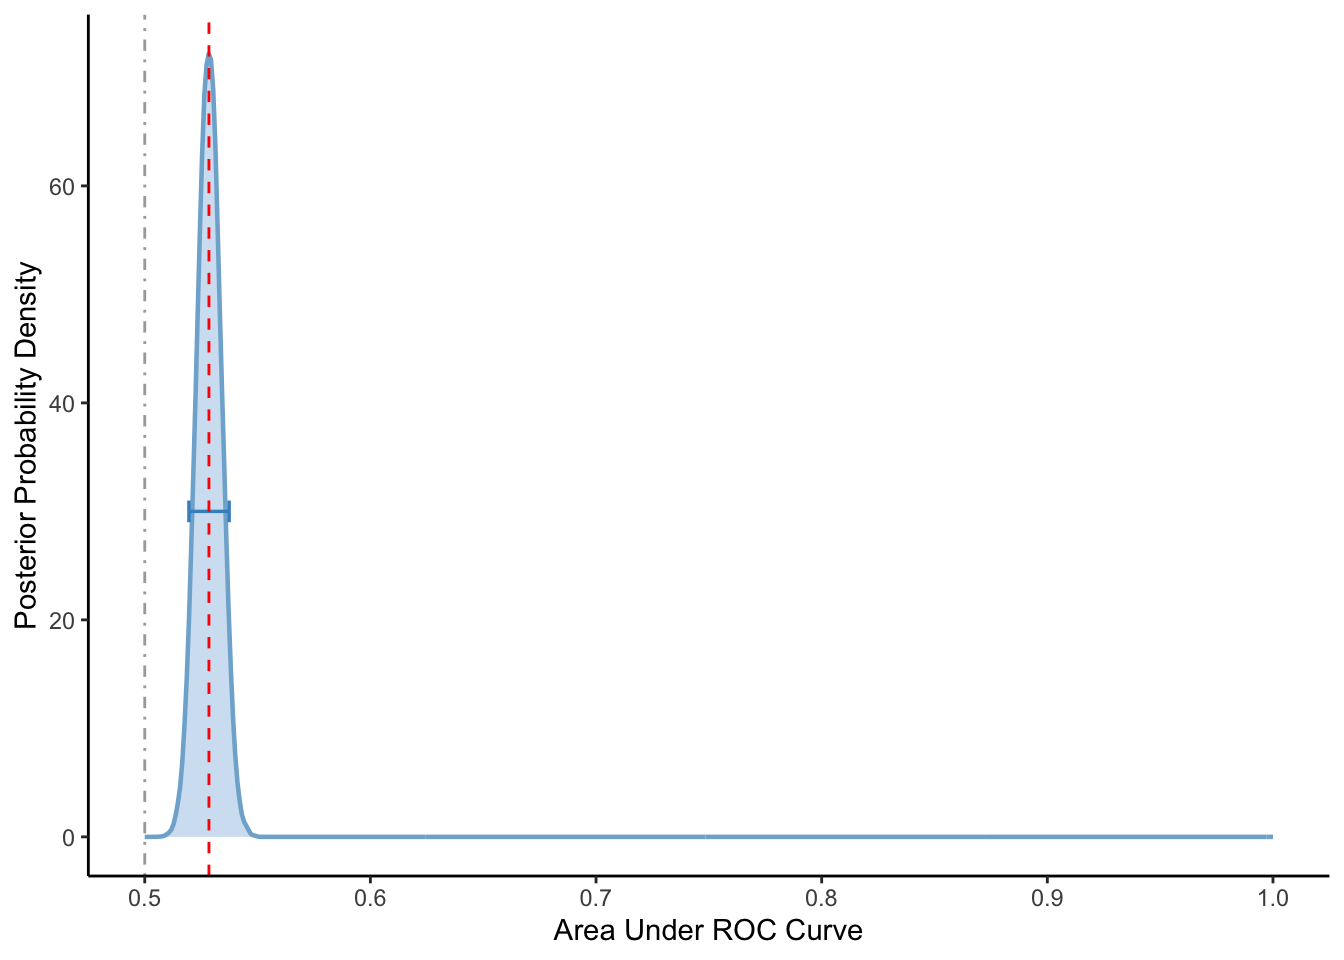
\includegraphics{index_files/figure-latex/notebooks-fig_auroc-fig-auroc_posterior-output-1.png}

}

\caption{\label{fig-auroc_posterior}Posterior Distribution of auROC
Scores}

\end{figure}%

\textsubscript{Source:
\href{https://jjcurtin.github.io/study_messages/notebooks/fig_auroc-preview.html\#cell-fig-auroc_posterior}{Performance
plots}}

\subsection{Model Fairness}\label{model-fairness}

73 (53\%) participants are females, 17 (12\%) are non-White minorities,
39 (28\%) earned less than half of the median income in Madison in Year
2017, and 13 (9\%) aged 55 or older (see Figure~\ref{fig-demographics}).
Our model performed consistently worse in unprivileged group
vs.~privileged group across all four demographic categories (see
Figure~\ref{fig-fairness} and Table~\ref{tbl-fairness}). The median of
posterior distribution of model performance difference was 0.03 (95\%CI
= {[}0.01, 0.06{]}) for White people compared to People of Color. The
probability of the performance for the White people higher than for
People of Color was 0.99. The posterior distribution of performance
differences also indicated that the model performed better in males than
in females (median = 0.02, 95\%CI = {[}0.01, 0.04{]}, probability =
1.00), in people younger than 55 than people older than 55 (median =
0.04, 95\%CI = {[}0.01, 0.07{]}, probability = 1.00), and in people that
have higher income than in those who have lower income (median = 0.02,
95\%CI = {[}0.00, 0.04{]}, probability = 0.99). We concluded that the
model performed significantly worse in unprivileged groups.

\begin{figure}[H]

\centering{

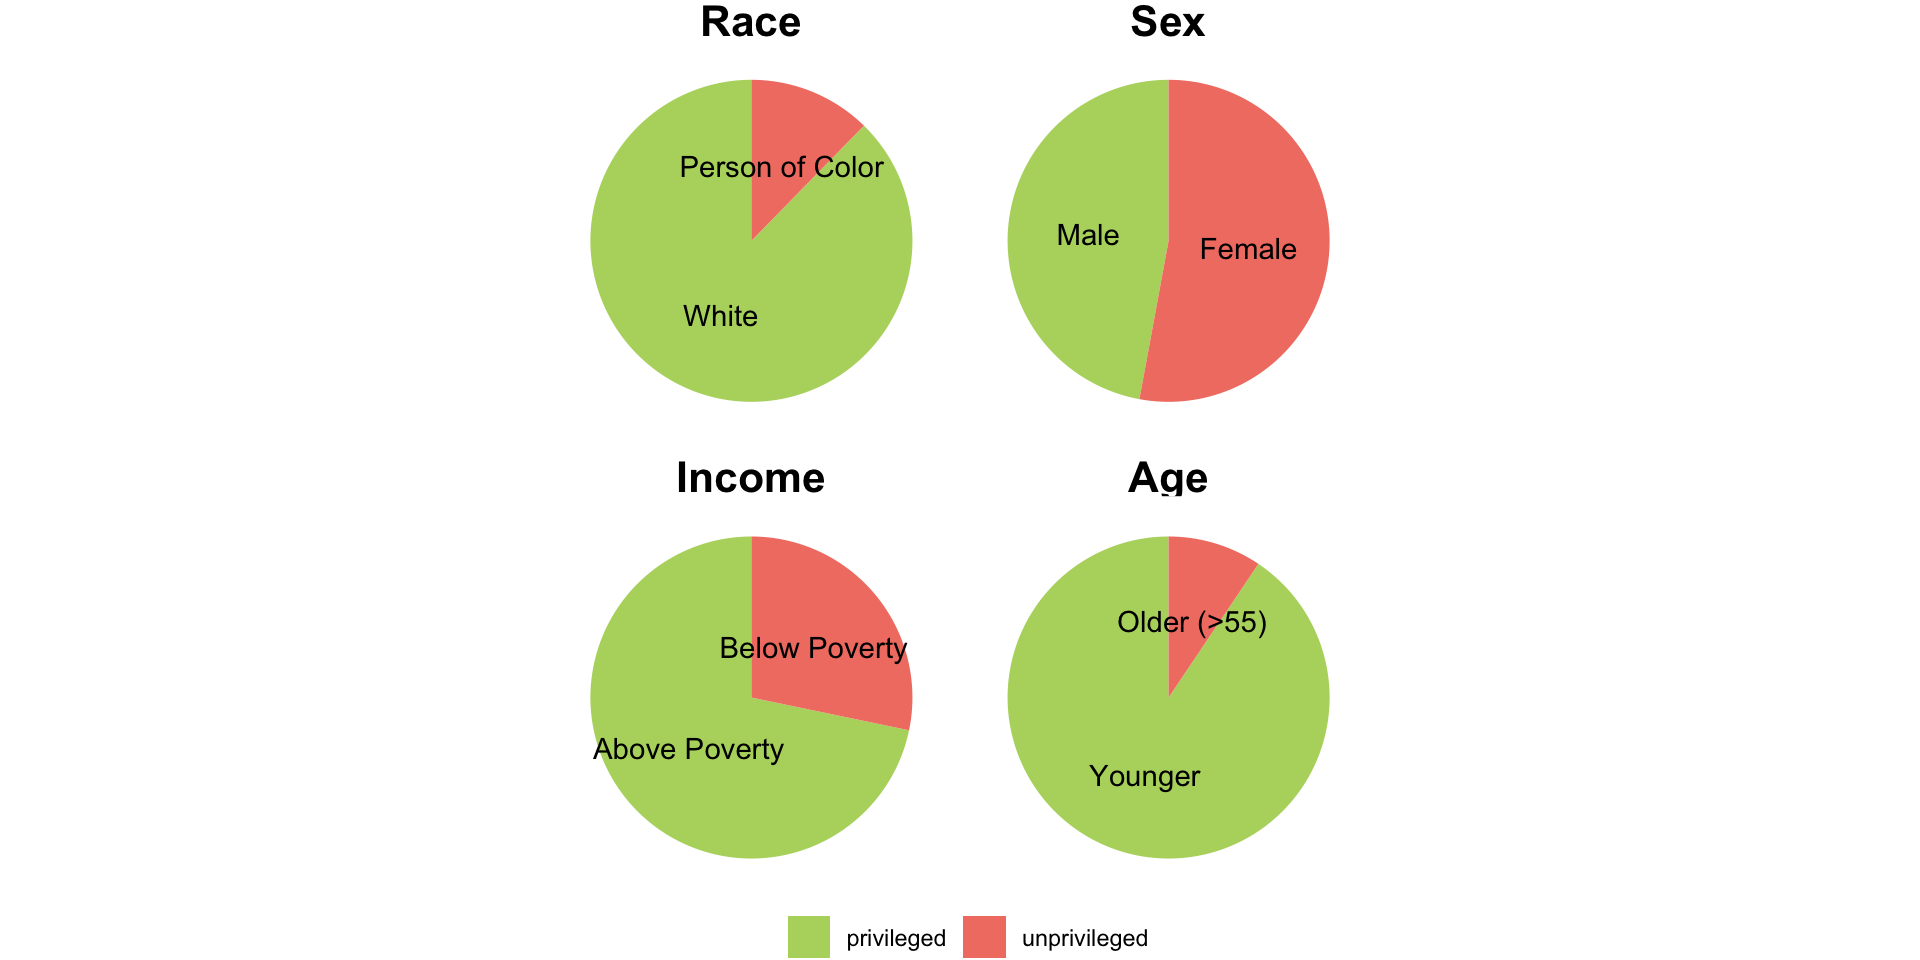
\includegraphics{index_files/figure-latex/notebooks-fig_demographics-fig-demographics-output-1.png}

}

\caption{\label{fig-demographics}Demographic Distribution}

\end{figure}%

\textsubscript{Source:
\href{https://jjcurtin.github.io/study_messages/notebooks/fig_demographics-preview.html\#cell-fig-demographics}{EDA
on Subject Demographics}}

\begin{figure}[H]

\centering{

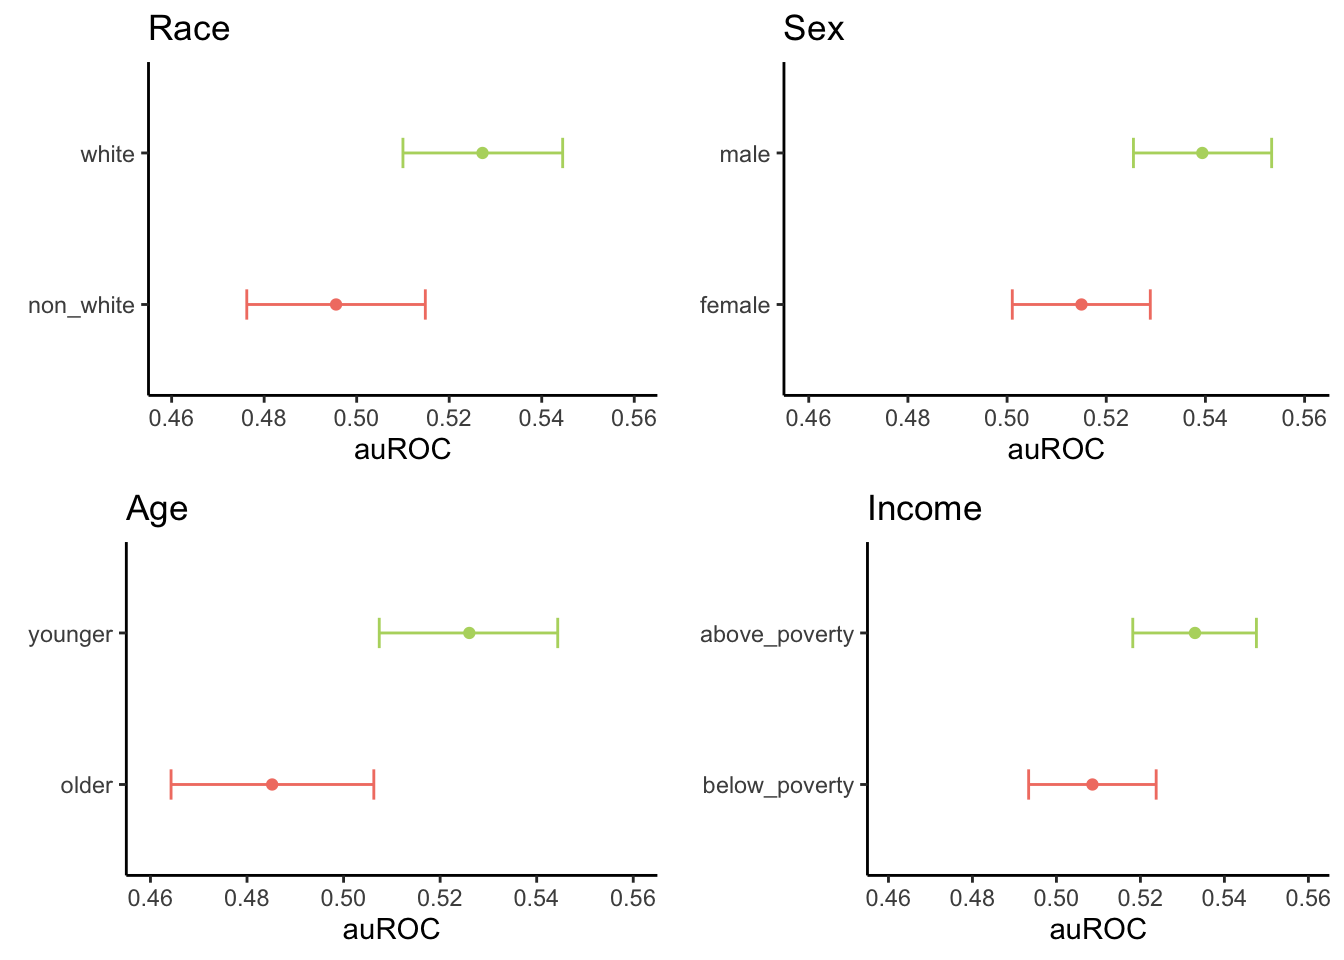
\includegraphics{index_files/figure-latex/notebooks-fig_fairness-fig-fairness-output-1.png}

}

\caption{\label{fig-fairness}auROC posterior distribution across
different privileged vs.~unprivileged groups}

\end{figure}%

\textsubscript{Source:
\href{https://jjcurtin.github.io/study_messages/notebooks/fig_fairness-preview.html\#cell-fig-fairness}{Subgroup
Analysis}}

\begin{longtable}[]{@{}
  >{\raggedright\arraybackslash}p{(\columnwidth - 8\tabcolsep) * \real{0.2000}}
  >{\raggedright\arraybackslash}p{(\columnwidth - 8\tabcolsep) * \real{0.2000}}
  >{\raggedright\arraybackslash}p{(\columnwidth - 8\tabcolsep) * \real{0.2000}}
  >{\raggedright\arraybackslash}p{(\columnwidth - 8\tabcolsep) * \real{0.2000}}
  >{\raggedright\arraybackslash}p{(\columnwidth - 8\tabcolsep) * \real{0.2000}}@{}}
\toprule\noalign{}
\begin{minipage}[b]{\linewidth}\raggedright
\end{minipage} & \begin{minipage}[b]{\linewidth}\raggedright
median
\end{minipage} & \begin{minipage}[b]{\linewidth}\raggedright
lower
\end{minipage} & \begin{minipage}[b]{\linewidth}\raggedright
upper
\end{minipage} & \begin{minipage}[b]{\linewidth}\raggedright
probability
\end{minipage} \\
\midrule\noalign{}
\endfirsthead
\toprule\noalign{}
\begin{minipage}[b]{\linewidth}\raggedright
\end{minipage} & \begin{minipage}[b]{\linewidth}\raggedright
median
\end{minipage} & \begin{minipage}[b]{\linewidth}\raggedright
lower
\end{minipage} & \begin{minipage}[b]{\linewidth}\raggedright
upper
\end{minipage} & \begin{minipage}[b]{\linewidth}\raggedright
probability
\end{minipage} \\
\midrule\noalign{}
\endhead
\bottomrule\noalign{}
\endlastfoot
white vs.~non\_white & 0.03 & 0.01 & 0.06 & 0.99 \\
male vs.~female & 0.02 & 0.01 & 0.04 & 1.00 \\
younger vs.~older & 0.04 & 0.01 & 0.07 & 1.00 \\
above\_poverty vs.~below\_poverty & 0.02 & 0.00 & 0.04 & 0.99 \\
\caption{Model Performance Difference across different demographic
subgroups}\label{tbl-fairness}\tabularnewline
\end{longtable}

\subsection{Model Interpretation}\label{model-interpretation}

The top 30 LIWC categories with the highest global shapley values were
displayed in Figure~\ref{fig-shaps}. Three categories appeared to be the
most robust in contributing to model output -- social processes (e.g.,
you, we, he, she), social behavior (e.g., said, love, say, care), and
second person pronoun (e.g., you, your, yourself). The other less robust
categories included total word count, clout (language of leadership),
assent (e.g., yeah, yes, okay, ok), social referents (e.g., you, we, he,
she), and prosocial behaviors (e.g., care, help, thank, please).

\begin{figure}[H]

\centering{

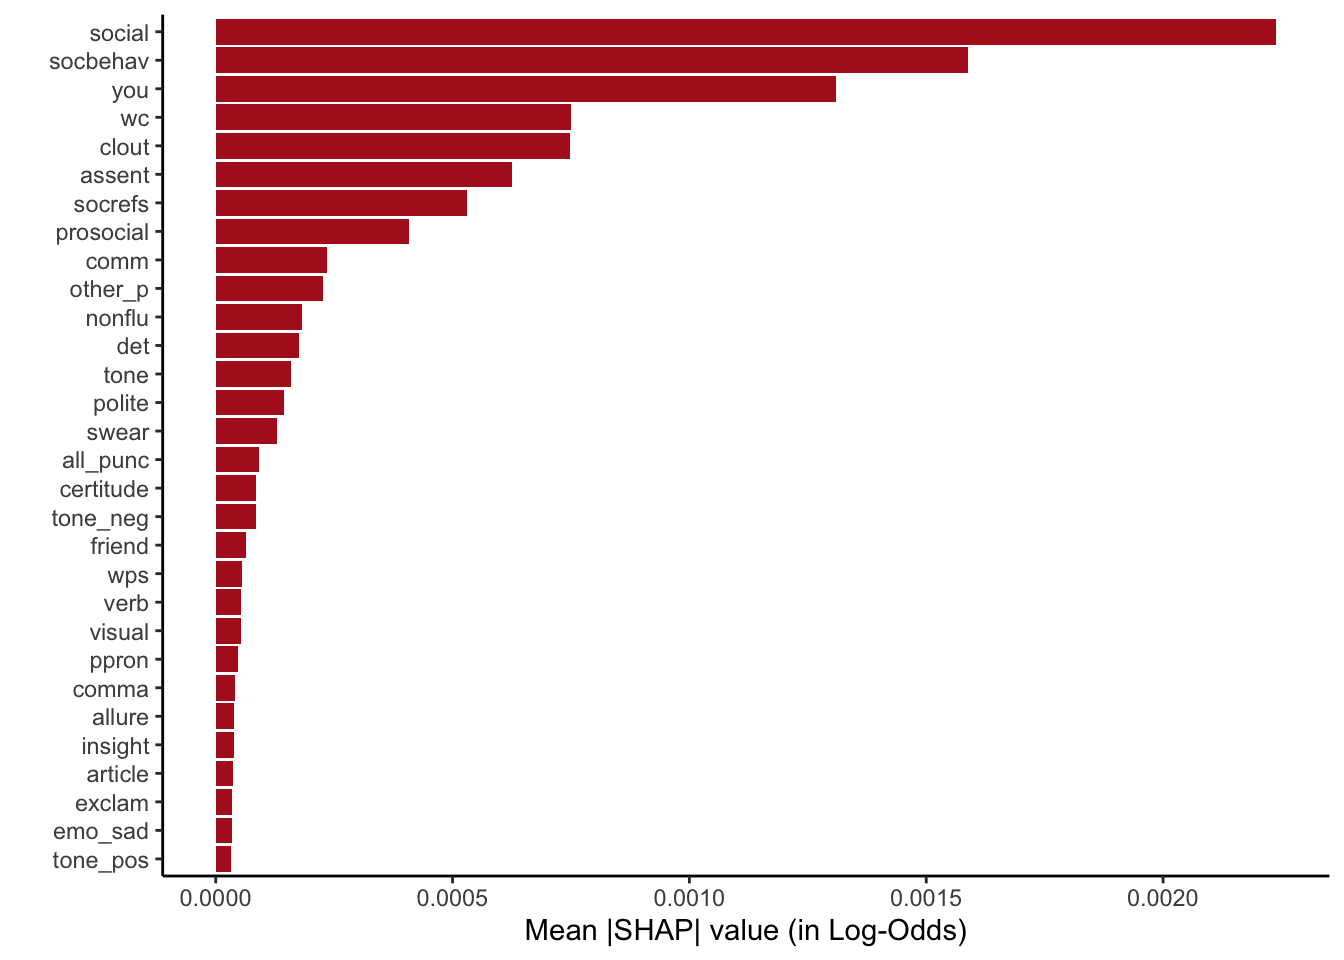
\includegraphics{index_files/figure-latex/notebooks-fig_shaps-fig-shaps-output-1.png}

}

\caption{\label{fig-shaps}Shapley Value}

\end{figure}%

\textsubscript{Source:
\href{https://jjcurtin.github.io/study_messages/notebooks/fig_shaps-preview.html\#cell-fig-shaps}{shaps}}

\newpage

\section{Discussion}\label{discussion}

Overall, our best machine learning model configuration leveraging
linguistic categories from SMS messages to predict a single episode of
alcohol lapse achieved an auROC score of .53. Our model was able to
extract signal from text messages. Nonetheless, the .03 increase beyond
chance performance is not sufficient enough for any clinical use.

Our LIWC model was only planned to serve as a baseline model against
which to later compare my sophisticated approaches following the FYP.
Clearly, more robust features need to be engineered from SMS messages to
achieve better prediction. Our next plan is to explore other more
sophisticated natural language processing (NLP) techniques to train our
models. In addition to the current configurations varying in prediction
window length, we might also incorporate configurations such as message
types.

To improve model performance, we might consider subsetting messages
based on their types. For instance, we can analyze incoming and outgoing
messages individually. By distinguishing between the two, we might get a
more refined understanding of communication dynamics. For example,
incoming messages might indicate the level of social support one gets
and outgoing messages might reflect their level of self-disclosure and
willingness to seek help. In the current study, we have taken a
different approach that combined the two message types together.
Although it provides an overview of social interactions between
participants and their contacts, it might overlook some nuanced
distinctions underlying texts from those two message types. On the other
hand, it is important to emphasize potential drawbacks to separate the
two message types, especially given the limited number of messages (see
\emph{Section Sample Distribution}) associated with each label. It might
lead to the problem of data sparsity which might even exacerbate model
performance and decrease its generalizability. We might consider
extended prediction window (e.g., 1-week window only) to aggregate more
data.

We can further try a variety of other natural language processing (NLP)
techniques for feature engineering including topic modeling, sentiment
analysis, n-grams approach and word embeddings. Our next and second
baseline model can be an n-grams approach. It represents bags-of-words
occurrences inside a document. We can leverage term frequency, inverse
document frequency and a combination of the two to mine word importance
inside a document. As this method yields high-dimensional data, we might
also consider combining it with dimension reduction approaches to do
feature engineering. Other NLP methods we might try include topic
modeling. It is an unsupervised machine learning methods to identify
clusters of topics in a body of text. We can also try other Sentiment
Analysis methods, beyond LIWC's native affect and emotion categories
which focus mostly on valence. For example, we might infer the emotional
underpinning of texts in terms of basic emotion categories (e.g., anger,
fear) from SMS messages. There are also other sentiment analysis
approaches outside of LIWC that can handle modifier words and provide
sentence level rather than word level analysis. We can also utilize word
embeddings---vectors that represent relationships of words within a
document in a lower-dimension.

Note that these feature engineering techniques differ in their
interpretability. Word embeddings is empirically-driven and its features
that are less interpretable. The interpretability of n-grams can depend
on the presence of words that contain high global importance. Topic
modeling, though data-driven, might yield topic clusters that are
interpretable. Sentiment Analysis can yield features that are highly
interpretable and might map on to current interventions. Importantly,
our desired predictive model should not just be the one that has the
highest predictive ability. We should also examine whether our model is
interpretable enough to understand intervention-relevant risk factors.
This helps us determine if our model can be clinically useful.

The minimal signal we detected in SMS messages might also reflect that
text messages itself is not an effective data source to predict lapses.
One potential reason might include that most people do not engage in
enough SMS texting behaviors that produce meaningful patterns near the
time of lapsing. Some people might also not use text messaging as their
main source of communication. Some might have preferences for texting in
other platforms (e.g., WhatsApp, Snapchat). The lack of sufficient data
points curtails machine learning models' ability to detect risk-relevant
signals. To enhance model performance, we might need increased access to
texts from other sources. Additionally, text messages might not convey
information indicative of risk-relevant factors such as alcohol cravings
(Korlakunta et al., 2012-07/2012-12; McKay, 1999; Wyant et al., 2024).
Communications in SMS messages might involve casual and monotonous
interactions which lacks specificity to effectively predict lapses.

Alternatively, we can explore adoption of metadata from text messages
and voice calls as predictive features. Those metadata include number of
messages within a prediction window, contextual information related to
the contact person, timing of messages or calls, etc. We can mine sudden
changes to messaging or calling behaviors from those metadata that might
signal enhanced lapse risks. For example, an increased number of late
night outgoing messages might indicate a sudden mood change preceding a
lapse. Note that we have already witnessed some success in our lab's
previous work (see Kendra's FYP), with auROCs in mid to upper .60s.

Surprisingly, despite the low performance score, we still witnessed
consistent unfairness in our algorithm for unprivileged demographic
subgroups. One key factor that contributed to the model biases might be
the disproportionate representation of subgroups such as racial
minorities. To address this limitation, we might recruit a sample with a
fair distribution of people with diverse backgrounds. Importantly,
however, our model still systematically misrepresented other demographic
subgroups even if they were well-represented in our training data. The
other explanation might be that our features were inherently biased
against subgroups. People from different demographic groups might
display different language styles, and LIWC might be more attuned to
those from the majority groups. As such, we should further try other
natural language processing techniques that incorporate more fair
features. For example, topic modeling does not rely on theories built
upon past, White male-dominated research and might yield more fair
features.

Results in this study indicate that text message might not be
potentially valuable raw data source in predicting alcohol lapses in AUD
patients. Although SMS messages offer the benefits of minimal burden on
users, this advantage cannot compensate for their low prediction
precision. EMA measures, despite their somewhat higher burden, are
capable of capturing robust signals. GPS sensing, which is also not
burdensome, can obtain some signals with little feature engineering (see
Claire's FYP). Note that both EMA and GPS sensing are easily accessible
across platforms. Nonetheless, as SMS is not currently available in ios
platform, we might have diminished further interest in this data source.

In sum, our machine learning algorithm had minimal increase in
performance compared to random guess. The results call for further
exploration of other feature engineering techniques to build models that
have higher performance, are interpretable and have low algorithmic
biases.

\newpage

\phantomsection\label{refs}
\begin{CSLReferences}{1}{0}
\bibitem[\citeproctext]{ref-abrahamAvailabilityMedicationsTreatment2020}
Abraham, A. J., Andrews, C. M., Harris, S. J., \& Friedmann, P. D.
(2020). Availability of {Medications} for the {Treatment} of {Alcohol}
and {Opioid Use Disorder} in the {USA}. \emph{Neurotherapeutics},
\emph{17}(1), 55--69. \url{https://doi.org/10.1007/s13311-019-00814-4}

\bibitem[\citeproctext]{ref-anderssonRelapseInpatientSubstance2019}
Andersson, H. W., Wenaas, M., \& Nordfjærn, T. (2019). Relapse after
inpatient substance use treatment: {A} prospective cohort study among
users of illicit substances. \emph{Addictive Behaviors}, \emph{90},
222--228. \url{https://doi.org/10.1016/j.addbeh.2018.11.008}

\bibitem[\citeproctext]{ref-beukenhorstUsingSmartphonesReduce2022a}
Beukenhorst, A. L., Burke, K. M., Scheier, Z., Miller, T. M., Paganoni,
S., Keegan, M., Collins, E., Connaghan, K. P., Tay, A., Chan, J., Berry,
J. D., \& Onnela, J.-P. (2022). Using smartphones to reduce research
burden in a neurodegenerative population and assessing participant
adherence: {A} randomized clinical trial and two observational studies.
\emph{JMIR Mhealth and Uhealth}, \emph{10}(2), e31877.
\url{https://doi.org/10.2196/31877}

\bibitem[\citeproctext]{ref-brownCharacteristicsRelapseFollowing1989}
Brown, S. A., Vik, P. W., \& Creamer, V. A. (1989). Characteristics of
relapse following adolescent substance abuse treatment. \emph{Addictive
Behaviors}, \emph{14}(3), 291--300.
\url{https://doi.org/10.1016/0306-4603(89)90060-9}

\bibitem[\citeproctext]{ref-bucciTheyAreNot2019}
Bucci, S., Berry, N., Morris, R., Berry, K., Haddock, G., Lewis, S., \&
Edge, D. (2019). {``{They Are Not Hard-to-Reach Clients}. {We Have Just
Got Hard-to-Reach Services}.''} {Staff Views} of {Digital Health Tools}
in {Specialist Mental Health Services}. \emph{Frontiers in Psychiatry},
\emph{10}. \url{https://doi.org/10.3389/fpsyt.2019.00344}

\bibitem[\citeproctext]{ref-chihPredictiveModelingAddiction2014a}
Chih, M.-Y., Patton, T., McTavish, F. M., Isham, A. J., Judkins-Fisher,
C. L., Atwood, A. K., \& Gustafson, D. H. (2014). Predictive modeling of
addiction lapses in a mobile health application. \emph{Journal of
Substance Abuse Treatment}, \emph{46}(1), 29--35.
\url{https://doi.org/10.1016/j.jsat.2013.08.004}

\bibitem[\citeproctext]{ref-chungRelapseAlcoholOther2006a}
Chung, T., \& Maisto, S. A. (2006). Relapse to alcohol and other drug
use in treated adolescents: {Review} and reconsideration of relapse as a
change point in clinical course. \emph{Clinical Psychology Review},
\emph{26}(2), 149--161. \url{https://doi.org/10.1016/j.cpr.2005.11.004}

\bibitem[\citeproctext]{ref-czyzEcologicalAssessmentDaily2018}
Czyz, E. K., King, C. A., \& Nahum-Shani, I. (2018). Ecological
assessment of daily suicidal thoughts and attempts among suicidal teens
after psychiatric hospitalization: {Lessons} about feasibility and
acceptability. \emph{Psychiatry Research}, \emph{267}, 566--574.
\url{https://doi.org/10.1016/j.psychres.2018.06.031}

\bibitem[\citeproctext]{ref-dibartoloAlcoholUseDisorder2017}
DiBartolo, M. C., \& Jarosinski, J. M. (2017). Alcohol {Use Disorder} in
{Older Adults}: {Challenges} in {Assessment} and {Treatment}.
\emph{Issues in Mental Health Nursing}, \emph{38}(1), 25--32.
\url{https://doi.org/10.1080/01612840.2016.1257076}

\bibitem[\citeproctext]{ref-finnPerceivedBarriersSeeking2023}
Finn, S. W., Mejldal, A., \& Nielsen, A. S. (2023). Perceived barriers
to seeking treatment for alcohol use disorders among the general
{Danish} population -- a cross sectional study on the role of severity
of alcohol use and gender. \emph{Archives of Public Health},
\emph{81}(1), 65. \url{https://doi.org/10.1186/s13690-023-01085-4}

\bibitem[\citeproctext]{ref-gilbertGenderDifferencesUse2019b}
Gilbert, P. A., Pro, G., Zemore, S. E., Mulia, N., \& Brown, G. (2019).
Gender {Differences} in {Use} of {Alcohol Treatment Services} and
{Reasons} for {Non-Use} in a {National Sample}. \emph{Alcoholism,
Clinical and Experimental Research}, \emph{43}(4), 722--731.
\url{https://doi.org/10.1111/acer.13965}

\bibitem[\citeproctext]{ref-gregoryFirstlineMedicationsOutpatient2022}
Gregory, C., Chorny, Y., McLeod, S. L., \& Mohindra, R. (2022).
First-line {Medications} for the {Outpatient Treatment} of {Alcohol Use
Disorder}: {A Systematic Review} of {Perceived Barriers}. \emph{Journal
of Addiction Medicine}.
\url{https://doi.org/10.1097/ADM.0000000000000918}

\bibitem[\citeproctext]{ref-gustafsonSmartphoneApplicationSupport2014b}
Gustafson, D. H., McTavish, F. M., Chih, M.-Y., Atwood, A. K., A.
Johnson, R., G. Boyle, M., S. Levy, M., Driscoll, H., M. Chisholm, S.,
Dillenburg, L., Isham, A., \& Shah, D. (2014). A smartphone application
to support recovery from alcoholism: {A} randomized controlled trial.
\emph{JAMA Psychiatry}, \emph{71}(5), 566--572.
\url{https://doi.org/10.1001/jamapsychiatry.2013.4642}

\bibitem[\citeproctext]{ref-hogstrombrandtPredictionSingleEpisodes1999a}
Högström Brandt, A. M., Thorburn, D., Hiltunen, A. J., \& Borg, S.
(1999). Prediction of single episodes of drinking during the treatment
of alcohol-dependent patients. \emph{Alcohol (Fayetteville, N.Y.)},
\emph{18}(1), 35--42.
\url{https://doi.org/10.1016/s0741-8329(98)00065-2}

\bibitem[\citeproctext]{ref-hungSmartphonebasedEcologicalMomentary2016}
Hung, S., Li, M.-S., Chen, Y.-L., Chiang, J.-H., Chen, Y.-Y., \& Hung,
G. C.-L. (2016). Smartphone-based ecological momentary assessment for
{Chinese} patients with depression: {An} exploratory study in {Taiwan}.
\emph{Asian Journal of Psychiatry}, \emph{23}, 131--136.
\url{https://doi.org/10.1016/j.ajp.2016.08.003}

\bibitem[\citeproctext]{ref-jacobsonRacialDisparitiesCompletion2007}
Jacobson, J. O., Robinson, P. L., \& Bluthenthal, R. N. (2007). Racial
{Disparities} in {Completion Rates} from {Publicly Funded Alcohol
Treatment}: {Economic Resources Explain More Than Demographics} and
{Addiction Severity}. \emph{Health Services Research}, \emph{42}(2),
773--794. \url{https://doi.org/10.1111/j.1475-6773.2006.00612.x}

\bibitem[\citeproctext]{ref-jacobsonUsingDigitalTherapeutics2023}
Jacobson, N., Quist, R., Lee, C., \& Marsch, L. (2023). \emph{Using
digital therapeutics to target gaps and failures in traditional mental
health and addiction treatments} (pp. 5--18).
\url{https://doi.org/10.1016/B978-0-323-90045-4.00005-8}

\bibitem[\citeproctext]{ref-kaddenMarlattRelapseTaxonomy1996}
Kadden, R. M. (1996). Is {Marlatt}'s relapse taxonomy reliable or valid?
\emph{Addiction}, \emph{91}(12s1), 139--146.
\url{https://doi.org/10.1046/j.1360-0443.91.12s1.4.x}

\bibitem[\citeproctext]{ref-kaufmannTreatmentSeekingBarriers2014}
Kaufmann, C. N., Chen, L.-Y., Crum, R. M., \& Mojtabai, R. (2014).
Treatment seeking and barriers to treatment for alcohol use in persons
with alcohol use disorders and comorbid mood or anxiety disorders.
\emph{Social Psychiatry and Psychiatric Epidemiology}, \emph{49}(9),
1489--1499. \url{https://doi.org/10.1007/s00127-013-0740-9}

\bibitem[\citeproctext]{ref-korlakuntaReasonsRelapsePatients2012}
Korlakunta, A., Chary, S. R. S., \& Reddy, P. K. C. (2012-07/2012-12).
Reasons for relapse in patients with alcohol dependence. \emph{Archives
of Mental Health}, \emph{13}(2), 108.

\bibitem[\citeproctext]{ref-lecomteMobileAppsMental2020}
Lecomte, T., Potvin, S., Corbière, M., Guay, S., Samson, C., Cloutier,
B., Francoeur, A., Pennou, A., \& Khazaal, Y. (2020). Mobile {Apps} for
{Mental Health Issues}: {Meta-Review} of {Meta-Analyses}. \emph{JMIR
mHealth and uHealth}, \emph{8}(5), e17458.
\url{https://doi.org/10.2196/17458}

\bibitem[\citeproctext]{ref-lowmanReplicationExtensionMarlatt1996a}
Lowman, C., Allen, J., Stout, R. L., \& Group, T. R. R. (1996).
Replication and extension of {Marlatt}'s taxonomy of relapse
precipitants: Overview of procedures and results. \emph{Addiction},
\emph{91}(12s1), 51--72.
\url{https://doi.org/10.1046/j.1360-0443.91.12s1.16.x}

\bibitem[\citeproctext]{ref-lundbergUnifiedApproachInterpreting2017}
Lundberg, S. M., \& Lee, S.-I. (2017). A unified approach to
interpreting model predictions. \emph{Proceedings of the 31st
{International Conference} on {Neural Information Processing Systems}},
4768--4777.

\bibitem[\citeproctext]{ref-mackesy-amitiFeasibilityEcologicalMomentary2018}
Mackesy-Amiti, M. E., \& Boodram, B. (2018). Feasibility of ecological
momentary assessment to study mood and risk behavior among young people
who inject drugs. \emph{Drug and Alcohol Dependence}, \emph{187},
227--235. \url{https://doi.org/10.1016/j.drugalcdep.2018.03.016}

\bibitem[\citeproctext]{ref-marlattTaxonomyHighriskSituations1996a}
Marlatt, G. A. (1996). Taxonomy of high-risk situations for alcohol
relapse: Evolution and development of a. \emph{Addiction},
\emph{91}(12s1), 37--50.
\url{https://doi.org/10.1046/j.1360-0443.91.12s1.15.x}

\bibitem[\citeproctext]{ref-marlattRelapsePreventionMaintenance2005a}
Marlatt, G. A., \& Donovan, D. M. (Eds.). (2005). \emph{Relapse
prevention: {Maintenance} strategies in the treatment of addictive
behaviors, 2nd ed} (pp. xiv, 416). The Guilford Press.

\bibitem[\citeproctext]{ref-mayBarriersTreatmentAlcohol2019}
May, C., Nielsen, A. S., \& Bilberg, R. (2019). Barriers to {Treatment}
for {Alcohol Dependence}. \emph{Journal of Drug and Alcohol Research},
\emph{8}(236083). \url{https://doi.org/10.4303/jdar/236083}

\bibitem[\citeproctext]{ref-mckayStudiesFactorsRelapse1999a}
McKay, J. R. (1999). Studies of factors in relapse to alcohol, drug and
nicotine use: A critical review of methodologies and findings.
\emph{Journal of Studies on Alcohol}, \emph{60}(4), 566--576.
\url{https://doi.org/10.15288/jsa.1999.60.566}

\bibitem[\citeproctext]{ref-mckayConceptualMethodologicalAnalytical2006b}
McKay, J. R., Franklin, T. R., Patapis, N., \& Lynch, K. G. (2006).
Conceptual, methodological, and analytical issues in the study of
relapse. \emph{Clinical Psychology Review}, \emph{26}(2), 109--127.
\url{https://doi.org/10.1016/j.cpr.2005.11.002}

\bibitem[\citeproctext]{ref-millerWhatRelapseFifty1996}
Miller, W. R. (1996). What is a relapse? {Fifty} ways to leave the
wagon. \emph{Addiction}, \emph{91}(12s1), 15--28.
\url{https://doi.org/10.1046/j.1360-0443.91.12s1.6.x}

\bibitem[\citeproctext]{ref-mogkImplementationWorkflowStrategies2023}
Mogk, J. M., Matson, T. E., Caldeiro, R. M., Garza Mcwethy, A. M.,
Beatty, T., Sevey, B. C., Hsu, C. W., \& Glass, J. E. (2023).
Implementation and workflow strategies for integrating digital
therapeutics for alcohol use disorders into primary care: {A}
qualitative study. \emph{Addiction Science \& Clinical Practice},
\emph{18}(1). \url{https://doi.org/10.1186/s13722-023-00387-w}

\bibitem[\citeproctext]{ref-nationalinstituteonalcoholabuseandalcoholismAlcoholTreatmentUnited2023}
National Institute on Alcohol Abuse and Alcoholism. (2023a).
\emph{Alcohol {Treatment} in the {United States} {\textbar} {National
Institute} on {Alcohol Abuse} and {Alcoholism} ({NIAAA})}.
https://www.niaaa.nih.gov/alcohols-effects-health/alcohol-topics/alcohol-facts-and-statistics/alcohol-treatment-united-states.

\bibitem[\citeproctext]{ref-nationalinstituteonalcoholabuseandalcoholismAlcoholUseDisorder2023}
National Institute on Alcohol Abuse and Alcoholism. (2023b).
\emph{Alcohol {Use Disorder} ({AUD}) in the {United States}: {Age
Groups} and {Demographic Characteristics} {\textbar} {National
Institute} on {Alcohol Abuse} and {Alcoholism} ({NIAAA})}.
https://www.niaaa.nih.gov/alcohols-effects-health/alcohol-topics/alcohol-facts-and-statistics/alcohol-use-disorder-aud-united-states-age-groups-and-demographic-characteristics.

\bibitem[\citeproctext]{ref-pennebakerDevelopmentPsychometricProperties2015a}
Pennebaker, J. W., Boyd, R. L., Jordan, K., \& Blackburn, K. (2015).
\emph{The {Development} and {Psychometric Properties} of {LIWC2015}}.

\bibitem[\citeproctext]{ref-philippeDigitalHealthInterventions2022}
Philippe, T. J., Sikder, N., Jackson, A., Koblanski, M. E., Liow, E.,
Pilarinos, A., \& Vasarhelyi, K. (2022). Digital {Health Interventions}
for {Delivery} of {Mental Health Care}: {Systematic} and {Comprehensive
Meta-Review}. \emph{JMIR Mental Health}, \emph{9}(5), e35159.
\url{https://doi.org/10.2196/35159}

\bibitem[\citeproctext]{ref-porras-segoviaSmartphonebasedEcologicalMomentary2020}
Porras-Segovia, A., Molina-Madueño, R. M., Berrouiguet, S.,
López-Castroman, J., Barrigón, M. L., Pérez-Rodríguez, M. S., Marco, J.
H., Díaz-Oliván, I., de León, S., Courtet, P., Artés-Rodríguez, A., \&
Baca-García, E. (2020). Smartphone-based ecological momentary assessment
({EMA}) in psychiatric patients and student controls: {A} real-world
feasibility study. \emph{Journal of Affective Disorders}, \emph{274},
733--741. \url{https://doi.org/10.1016/j.jad.2020.05.067}

\bibitem[\citeproctext]{ref-probstAlcoholUseDisorder2015}
Probst, C., Manthey, J., Martinez, A., \& Rehm, J. (2015). Alcohol use
disorder severity and reported reasons not to seek treatment: A
cross-sectional study in {European} primary care practices.
\emph{Substance Abuse Treatment, Prevention, and Policy}, \emph{10}(1),
32. \url{https://doi.org/10.1186/s13011-015-0028-z}

\bibitem[\citeproctext]{ref-sacks2010NationalState2015a}
Sacks, J. J., Gonzales, K. R., Bouchery, E. E., Tomedi, L. E., \&
Brewer, R. D. (2015). 2010 {National} and {State Costs} of {Excessive
Alcohol Consumption}. \emph{American Journal of Preventive Medicine},
\emph{49}(5), e73--e79.
\url{https://doi.org/10.1016/j.amepre.2015.05.031}

\bibitem[\citeproctext]{ref-schulerPerceivedBarriersTreatment2015}
Schuler, M. S., Puttaiah, S., Mojtabai, R., \& Crum, R. M. (2015).
Perceived {Barriers} to {Treatment} for {Alcohol Problems}: {A Latent
Class Analysis}. \emph{Psychiatric Services}, \emph{66}(11), 1221--1228.
\url{https://doi.org/10.1176/appi.ps.201400160}

\bibitem[\citeproctext]{ref-scottPathwaysRelapseTreatment2005}
Scott, C. K., Foss, M. A., \& Dennis, M. L. (2005). Pathways in the
relapse--treatment--recovery cycle over 3 years. \emph{Journal of
Substance Abuse Treatment}, \emph{28 Suppl 1}, S63--72.
\url{https://doi.org/10.1016/j.jsat.2004.09.006}

\bibitem[\citeproctext]{ref-sedarousCultureStigmaInequities2023}
Sedarous, M., \& Flemming, J. A. (2023). Culture, stigma, and inequities
creating barriers in alcohol use disorder management in
alcohol-associated liver disease. \emph{Clinical Liver Disease},
\emph{21}(5), 130. \url{https://doi.org/10.1097/CLD.0000000000000026}

\bibitem[\citeproctext]{ref-stoutPredictiveValidityMarlatt1996}
Stout, R. L., Longabaugh, R., \& Rubin, A. (1996). Predictive validity
of {Marlatt}'s relapse taxonomy versus a more general relapse code.
\emph{Addiction}, \emph{91}(12s1), 99--110.
\url{https://doi.org/10.1046/j.1360-0443.91.12s1.20.x}

\bibitem[\citeproctext]{ref-vangenugtenExperiencedBurdenAdherence2020a}
van Genugten, C. R., Schuurmans, J., Lamers, F., Riese, H., Penninx, B.
W. J. H., Schoevers, R. A., Riper, H. M., \& Smit, J. H. (2020).
Experienced {Burden} of and {Adherence} to {Smartphone-Based Ecological
Momentary Assessment} in {Persons} with {Affective Disorders}.
\emph{Journal of Clinical Medicine}, \emph{9}(2), 322.
\url{https://doi.org/10.3390/jcm9020322}

\bibitem[\citeproctext]{ref-verissimoInfluenceGenderRace2017}
Verissimo, A. D. O., \& Grella, C. E. (2017). Influence of gender and
race/ethnicity on perceived barriers to help-seeking for alcohol or drug
problems. \emph{Journal of Substance Abuse Treatment}, \emph{75},
54--61. \url{https://doi.org/10.1016/j.jsat.2016.12.013}

\bibitem[\citeproctext]{ref-wallhedfinnAlcoholConsumptionDependence2014}
Wallhed Finn, S., Bakshi, A.-S., \& Andréasson, S. (2014). Alcohol
{Consumption}, {Dependence}, and {Treatment Barriers}: {Perceptions
Among Nontreatment Seekers} with {Alcohol Dependence}. \emph{Substance
Use \& Misuse}, \emph{49}(6), 762--769.
\url{https://doi.org/10.3109/10826084.2014.891616}

\bibitem[\citeproctext]{ref-williamsBarriersFacilitatorsAlcohol2018}
Williams, E. C., Achtmeyer, C. E., Young, J. P., Berger, D., Curran, G.,
Bradley, K. A., Richards, J., Siegel, M. B., Ludman, E. J., Lapham, G.
T., Forehand, M., \& Harris, A. H. S. (2018). Barriers to and
{Facilitators} of {Alcohol Use Disorder Pharmacotherapy} in {Primary
Care}: {A Qualitative Study} in {Five VA Clinics}. \emph{Journal of
General Internal Medicine}, \emph{33}(3), 258--267.
\url{https://doi.org/10.1007/s11606-017-4202-z}

\bibitem[\citeproctext]{ref-witkiewitzRelapsePreventionAlcohol2004b}
Witkiewitz, K., \& Marlatt, G. A. (2004). Relapse prevention for alcohol
and drug problems: That was {Zen}, this is {Tao}. \emph{The American
Psychologist}, \emph{59}(4), 224--235.
\url{https://doi.org/10.1037/0003-066X.59.4.224}

\bibitem[\citeproctext]{ref-witkiewitzModelingComplexityPosttreatment2007a}
Witkiewitz, K., \& Marlatt, G. A. (2007). Modeling the complexity of
post-treatment drinking: {It}'s a rocky road to relapse. \emph{Clinical
Psychology Review}, \emph{27}(6), 724--738.
\url{https://doi.org/10.1016/j.cpr.2007.01.002}

\bibitem[\citeproctext]{ref-wyantAcceptabilityPersonalSensing2023a}
Wyant, K., Moshontz, H., Ward, S. B., Fronk, G. E., \& Curtin, J. J.
(2023). Acceptability of {Personal Sensing Among People With Alcohol Use
Disorder}: {Observational Study}. \emph{JMIR mHealth and uHealth},
\emph{11}, e41833. \url{https://doi.org/10.2196/41833}

\bibitem[\citeproctext]{ref-wyantMachineLearningModels2024}
Wyant, K., Sant'Ana, S. J., Fronk, G. E., \& Curtin, J. J. (2024).
Machine learning models for temporally precise lapse prediction in
alcohol use disorder. \emph{Journal of Psychopathology and Clinical
Science}, \emph{133}(7), 527--540.
\url{https://doi.org/10.1037/abn0000901}

\bibitem[\citeproctext]{ref-youngDifferencesPerceptionsPractices2018}
Young, J. P., Achtmeyer, C. E., Bensley, K. M., Hawkins, E. J., \&
Williams, E. C. (2018). Differences in {Perceptions} of and {Practices
Regarding Treatment} of {Alcohol Use Disorders Among VA Primary Care
Providers} in {Urban} and {Rural Clinics}. \emph{The Journal of Rural
Health}, \emph{34}(4), 359--368. \url{https://doi.org/10.1111/jrh.12293}

\end{CSLReferences}




\end{document}
